\def\paperTitle{Lab 2}
\def\paperSubTitle{RC Circuit Phase Shift}

\documentclass[
	12pt,twoside,a4paper
]{report}

\usepackage{graphicx}
\usepackage[margin=1in]{geometry}
\usepackage{fancyhdr}
\usepackage[utf8]{inputenc}
\usepackage{etoc}
\usepackage{xcolor, soul}
\usepackage{listings}
\usepackage{amsmath}
\usepackage{lipsum}
\usepackage{pgfplots}
\usepackage{hyperref}
\usepackage{tikz}
\usepackage{circuitikz}
\usepackage{subcaption}

\sethlcolor{yellow}

\fancypagestyle{plain}{
	\fancyhf{}
	\fancyhead[l]{\paperTitle}
	\fancyhead[c]{\paperSubTitle}
	\fancyhead[r]{October 21, 2024}
	\fancyfoot[le, ro]{Page \thepage}
	\fancyfoot[re, lo]{EE212}
	\setlength{\headheight}{15pt}
	\renewcommand{\headrulewidth}{0.2pt}
	\renewcommand{\footrulewidth}{0.2pt}
}	

\thispagestyle{plain}

\renewcommand{\etocaftertitlehook}{\thispagestyle{plain}}
\renewcommand{\etocaftertochook}{\thispagestyle{plain}}

\begin{document}
	\begin{center}
	
\includegraphics[width=0.4\textwidth]{assets/agu.png}

	\Huge
	\textbf{Abdullah Gül University}
	
	\vspace{0.3cm}
	Department of Electrical and Electronics Engineering

	\vspace{1cm}
	\Huge
	\textbf{\paperTitle}

	\vspace{0.3cm}
	\Huge
	\paperSubTitle{}

	\vspace{0.8cm}
	\large
	\vspace{0.5cm}
	\LARGE
	\vspace{1.5cm}
	\textbf{}
	\vfill
	\vspace{0.8cm}
	\Large
\end{center}

\begin{tabbing}
	\hspace*{1em}\= \hspace*{8em} \= \kill
	\> Barış DEMİRCİ \> agu@338.rocks \\
	\> \> \\
	\> October 13, 2024 \> \\
\end{tabbing}

	\tableofcontents

	\chapter{Overview}

\section{Objective}
The purpose of this lab is to understand the behavior of operational amplifiers (a.k.a op-amps) by conducting AC Sweep/Noise analysis, plotting input-output graphs at varying frequencies, and designing a non-inverting amplifier circuit with a gain of $4$. 

\section{Equipment}
\begin{itemize}
    \item Breadboard
    \item Oscilloscope
    \item Function Generator
    \item Multimeter
    \item LM741 Op-Amp
    \item Resistors ($1k\Omega$, $10k\Omega$)
    \item Capacitor ($100nF$)
\end{itemize}

	\chapter{Procedure}

\section{RLC Circuit Analysis}

\subsection{Theoretical Analysis}

\subsubsection{Transfer Function Derivation}
In order to derive the voltage gain transfer function ($H_{V}(s)$), we must first convert the circuit from time domain to the s-domain. The circuit is shown in Figure \ref{fig:rlc_circuit}.

\begin{figure}[h]
    \centering
    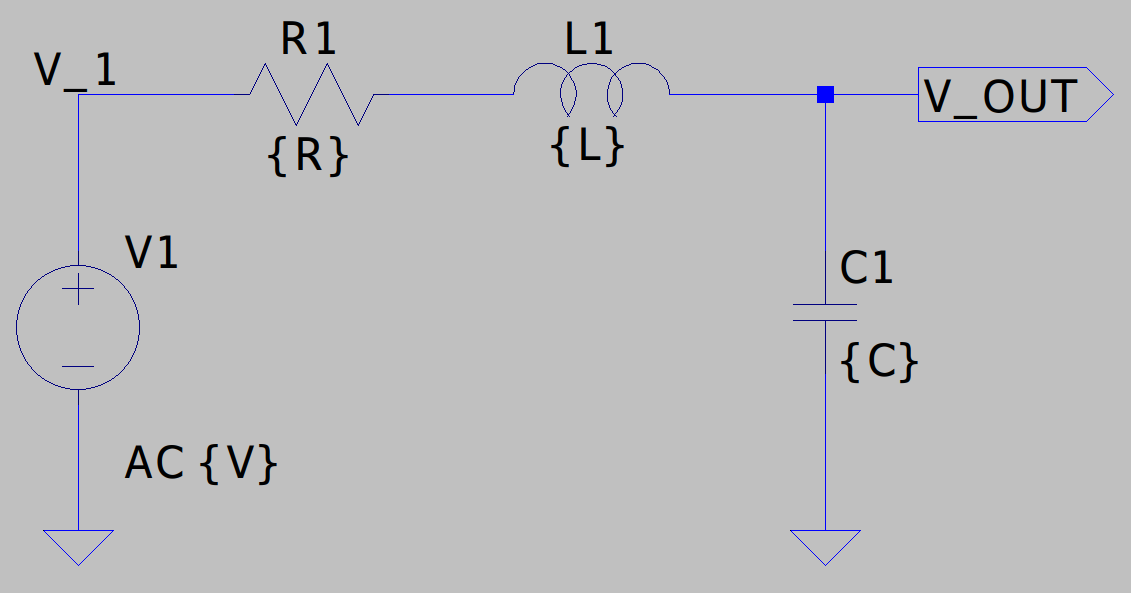
\includegraphics[width=0.8\textwidth]{assets/rlc-circ.png}
    \caption{RLC Circuit}
    \label{fig:rlc_circuit}
\end{figure}

\noindent Where:
\begin{itemize}
    \item $V_{1}$ is $1 V_{pp}$ input voltage.
    \item $V_{out}$ is the output voltage.
    \item $R$ is $1k\Omega$ resistor.
    \item $L$ is $1mH$ inductor.
    \item $C$ is $0.1\mu F$ capacitor.
\end{itemize}

\newpage
\thispagestyle{plain}

To find the transfer function, we first transform the circuit to the s-domain. The impedance of the resistor, inductor, and capacitor are given by:
\begin{align*}
    Z_{R} &= R \\
    Z_{L} &= sL \\
    Z_{C} &= \frac{1}{sC}
\end{align*}

And the KVL equation for the circuit is:
\begin{align*}
    V_{1} &= V_{R} + V_{L} + V_{C} \\
    V_{1} &= IZ_{R} + IZ_{L} + IZ_{C} \\
    V_{1} &= I(R + sL + \frac{1}{sC}) \\
\end{align*}

Where $I$ is the current through the circuit. The voltage gain transfer function is then:
\begin{align*}
    H_{V}(s) = \frac{V_{out}}{V_{1}} &= \frac{I\frac{1}{sC}}{I(R + sL + \frac{1}{sC})} \\
    &= \frac{\frac{1}{sC}}{R + sL + \frac{1}{sC}} \\
    &\boxed{H_{V}(s) = \frac{1}{sRC + s^{2}LC + 1}}
\end{align*}

\subsubsection{AC Sweep Analysis Simulation}
To validate the transfer function, we will perform an AC Sweep analysis in LTSpice. The AC Sweep analysis will sweep the frequency of the input voltage from $101Hz$ to $120kHz$. The output voltage will be measured and compared to the transfer function.

\begin{figure}[h]
    \centering
    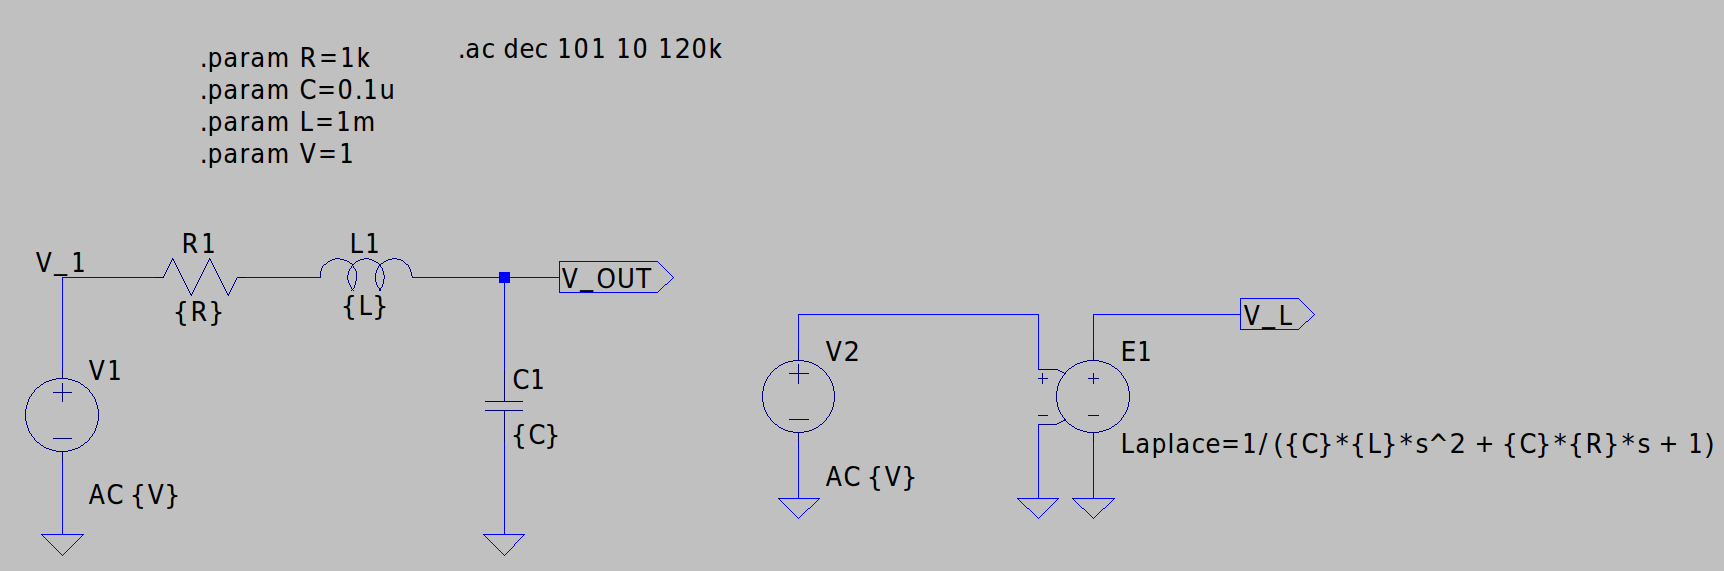
\includegraphics[width=1\textwidth, height=0.3\textheight]{assets/rlc-sim.png}
    \caption{AC Sweep Analysis Simulation Setup}
    \label{fig:ac_sweep}
\end{figure}


\newpage
\thispagestyle{plain}

\begin{figure}[h]
    \centering
    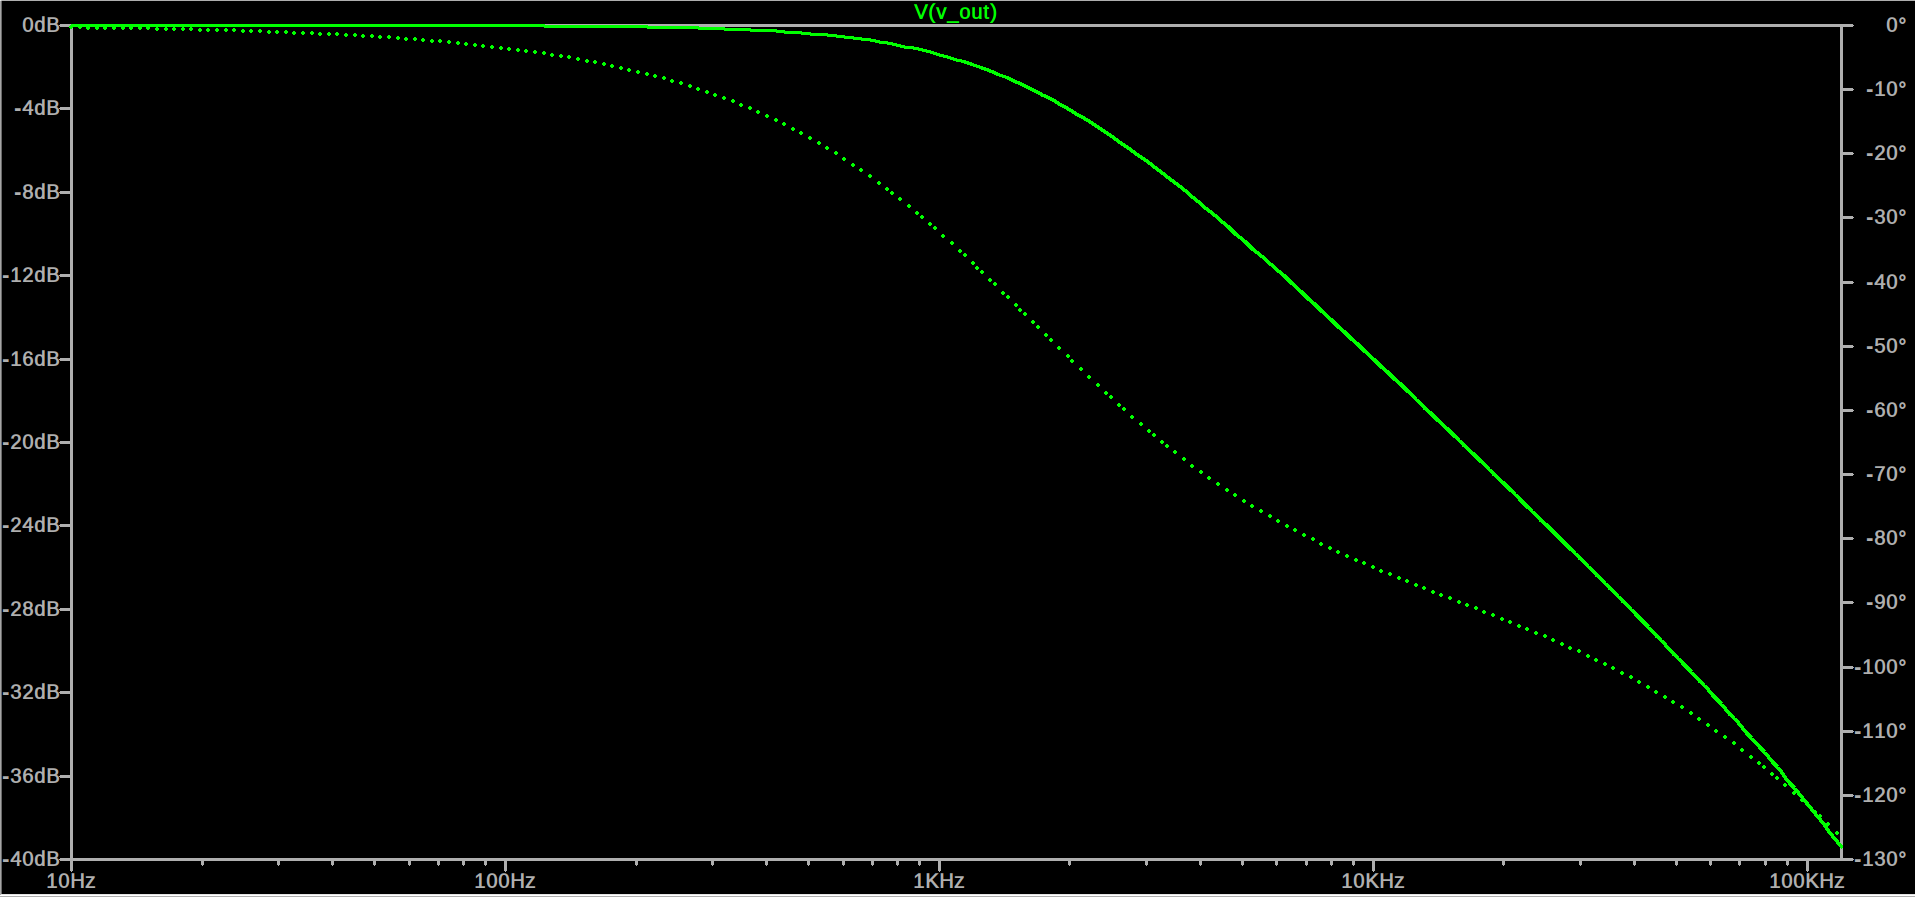
\includegraphics[width=1\textwidth]{assets/rlc-v-out.png}
    \caption{$V_{out}$ Bode Plot}
    \label{fig:rlc_v_out_bode_plot}
\end{figure}
\begin{figure}[h]
    \centering
    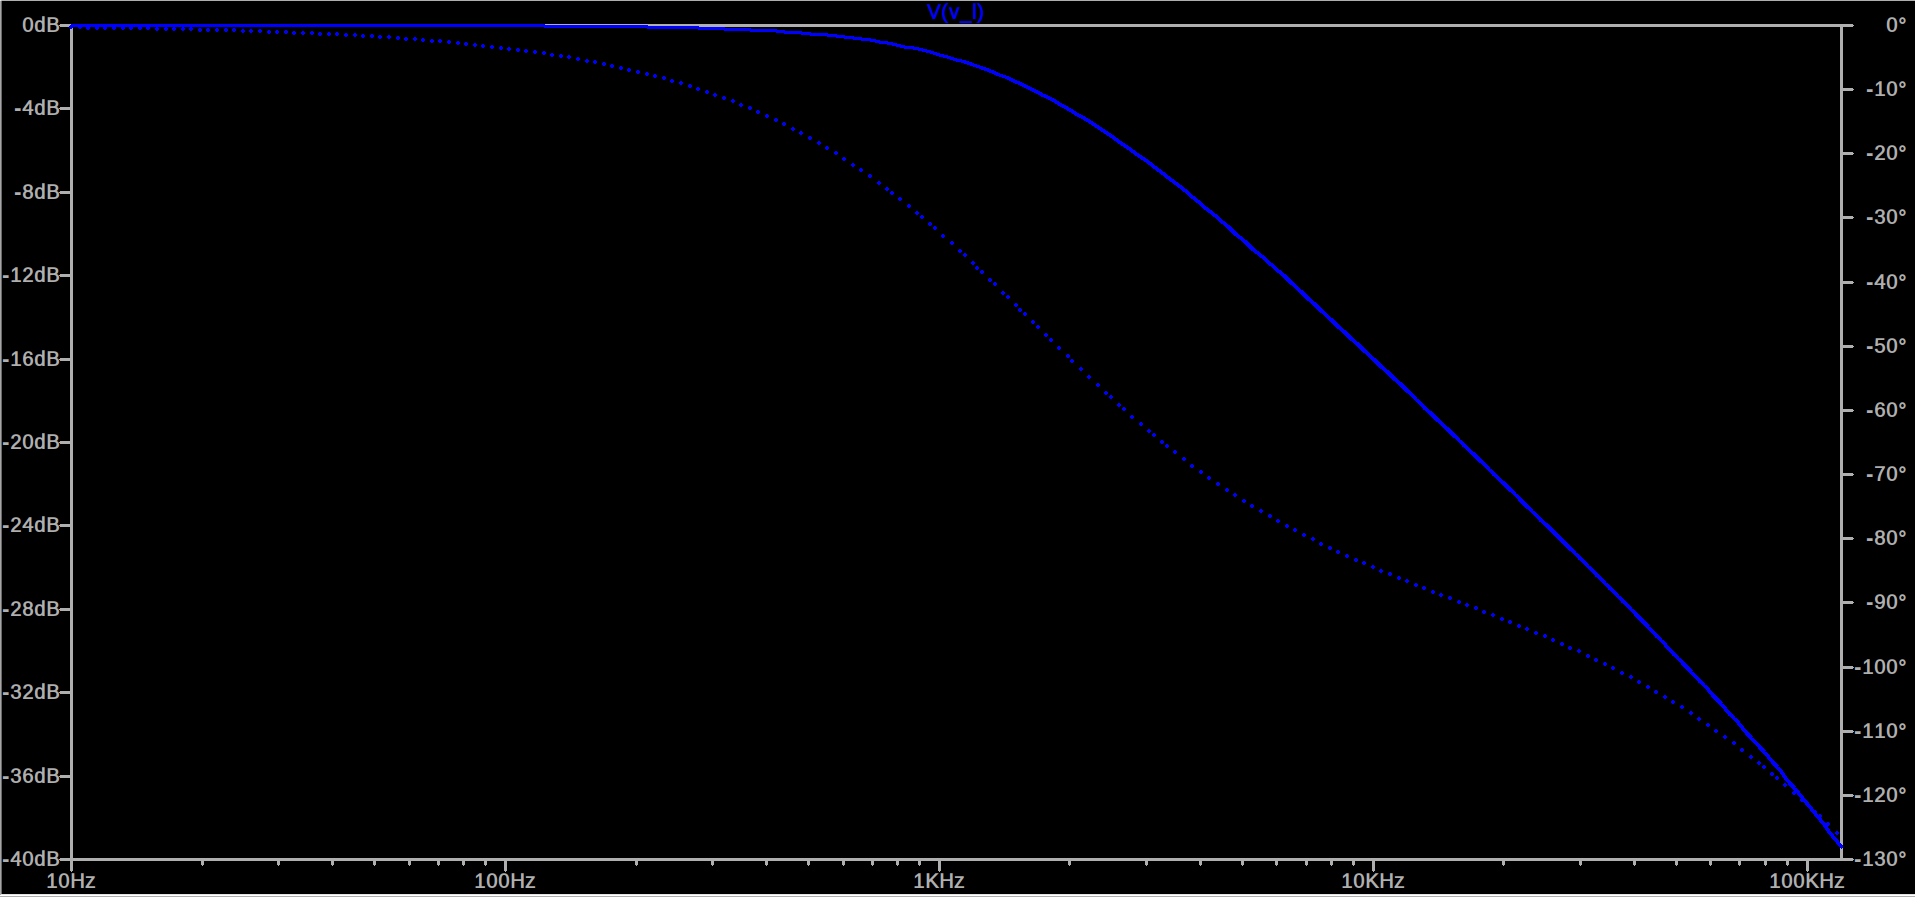
\includegraphics[width=1\textwidth]{assets/rlc-v-l.png}
    \caption{$H_{V}(s)$ Bode Plot}
    \label{fig:rlc_v_laplace_bode_plot}
\end{figure}

As shown in Figure \ref{fig:rlc_v_out_bode_plot}, output voltage frequency response matches the transfer function $H_{V}(s)$ as shown in Figure \ref{fig:rlc_v_laplace_bode_plot}.

\newpage
\thispagestyle{plain}

\subsubsection{Transient Analysis Simulation}
To further validate the transfer function, we will perform a transient analysis in LTSpice. Changed the input voltage $V_{ac}$ to a $1V_{pp}$ sine wave at $10kHz$. The output voltage will be measured and compared to the transfer function.

\begin{figure}[h]
    \centering
    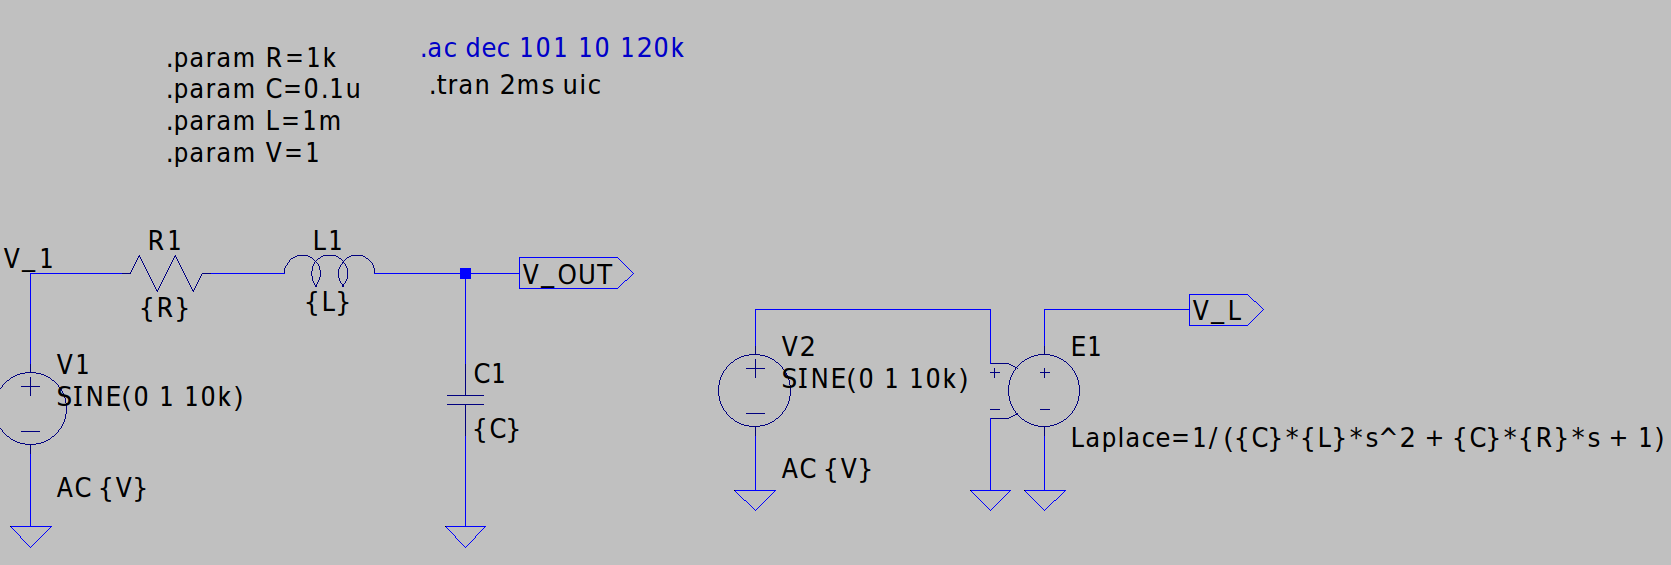
\includegraphics[width=1\textwidth, height=0.4\textheight]{assets/rlc-transient-sim.png}
    \caption{Transient Analysis Simulation Setup}
    \label{fig:transient_analysis}
\end{figure}

\newpage
\thispagestyle{plain}

\begin{figure}[h]
    \centering
    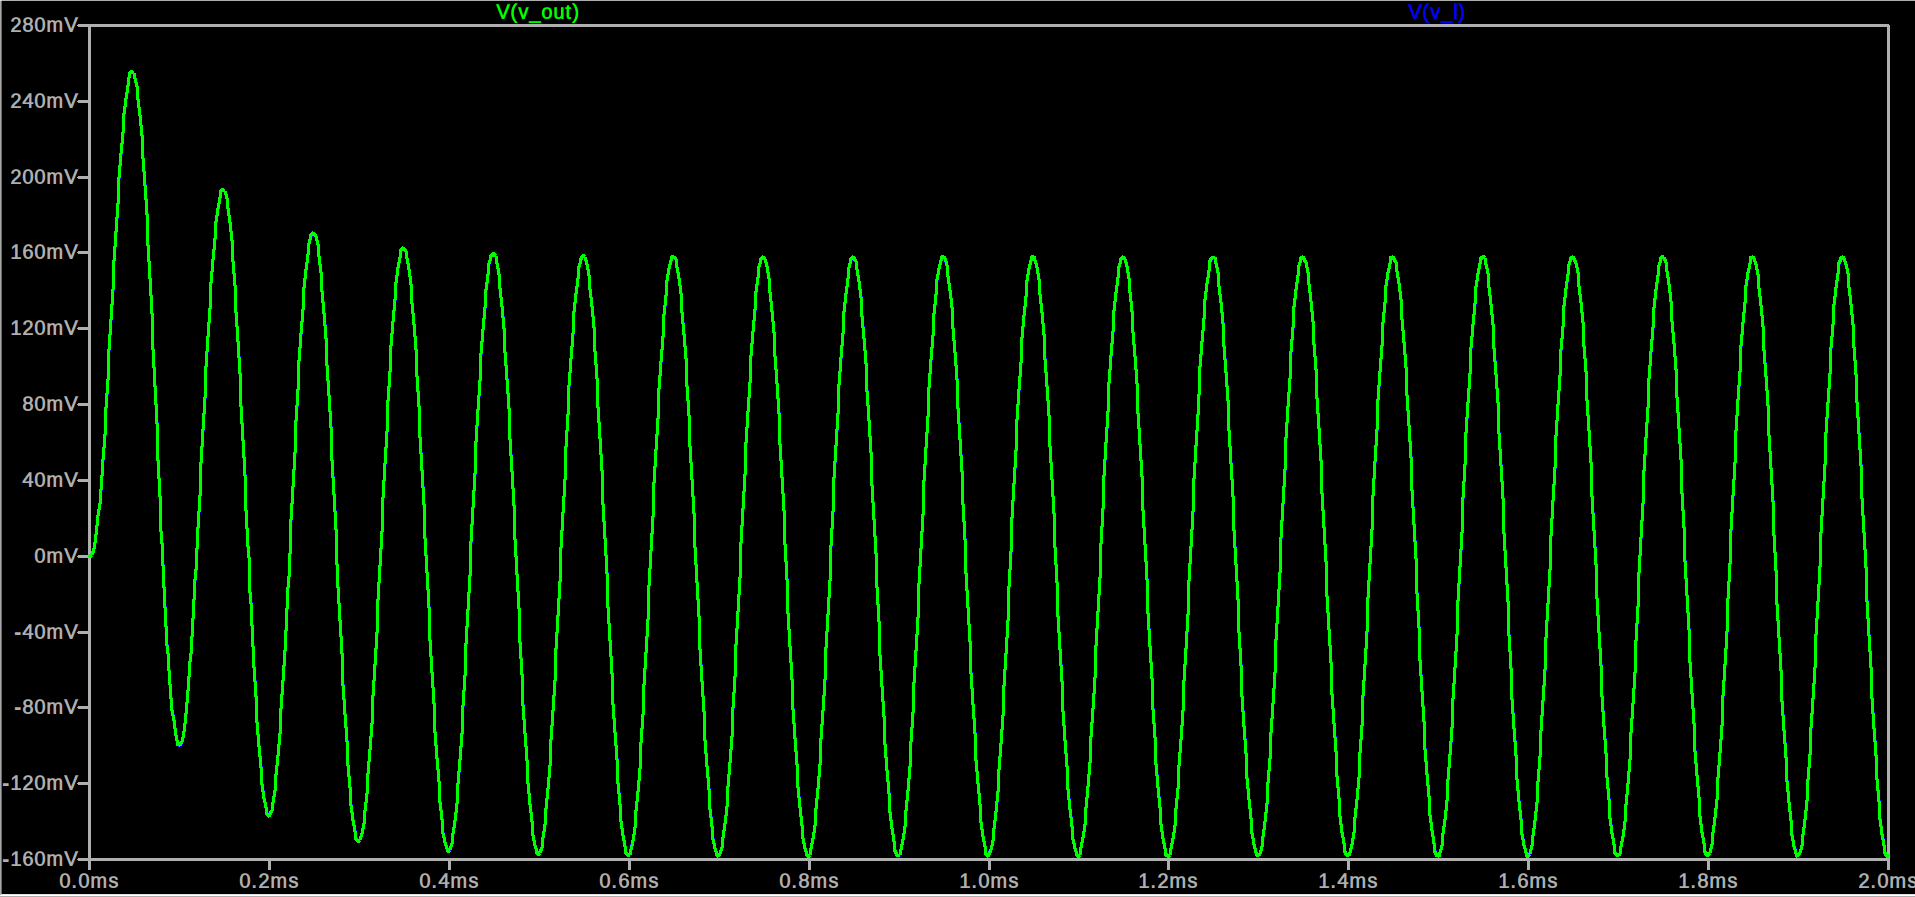
\includegraphics[width=1\textwidth]{assets/rlc-sin-transient-out.png}
    \caption{$V_{out}$ Transient Response}
    \label{fig:rlc_v_out_transient}
\end{figure}

\begin{figure}[h]
    \centering
    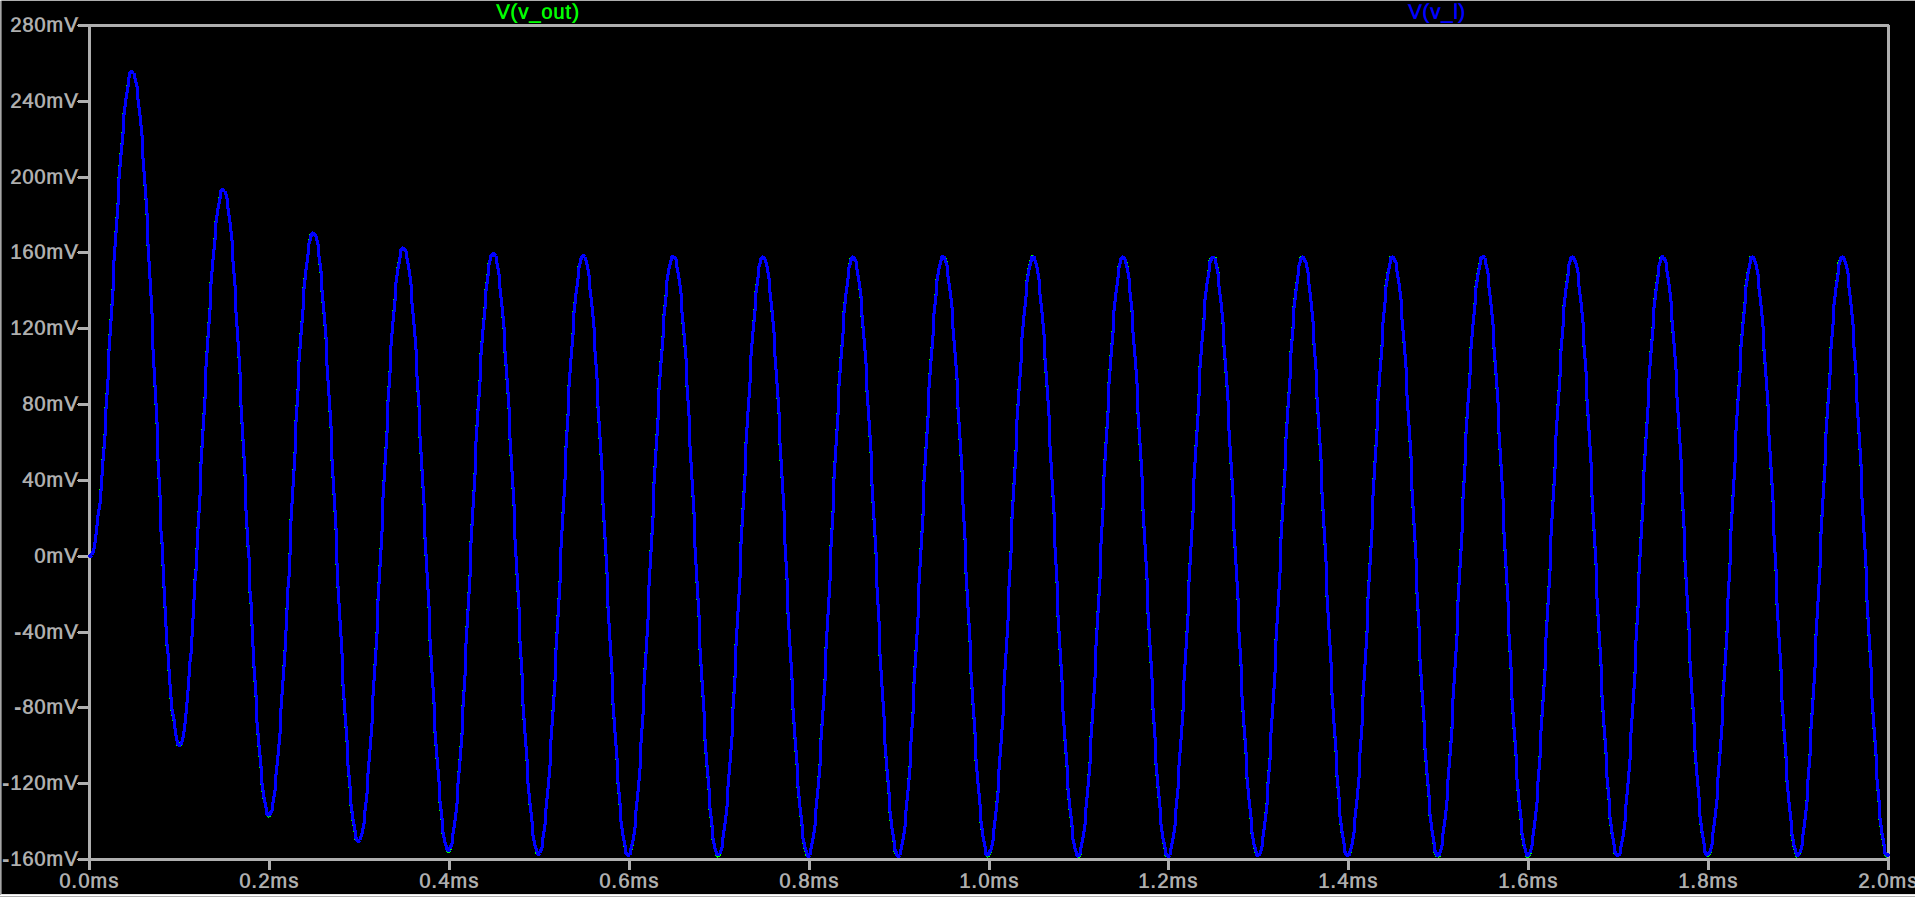
\includegraphics[width=1\textwidth]{assets/rlc-sin-transient-laplace.png}
    \caption{$H_{V}(s)$ Transient Response}
    \label{fig:rlc_v_laplace_transient}
\end{figure}

As shown in Figure \ref{fig:rlc_v_out_transient}, output voltage matches the transfer function $H_{V}(s)$ as shown in Figure \ref{fig:rlc_v_laplace_transient}.

\newpage
\thispagestyle{plain}

\subsubsection{Unit Step Response}
Unit step response can show the transient behavior of the circuit. In order to find unit step response, Heaviside step function ($u(t)$) is used as input voltage.

\begin{figure}[h]
    \centering
    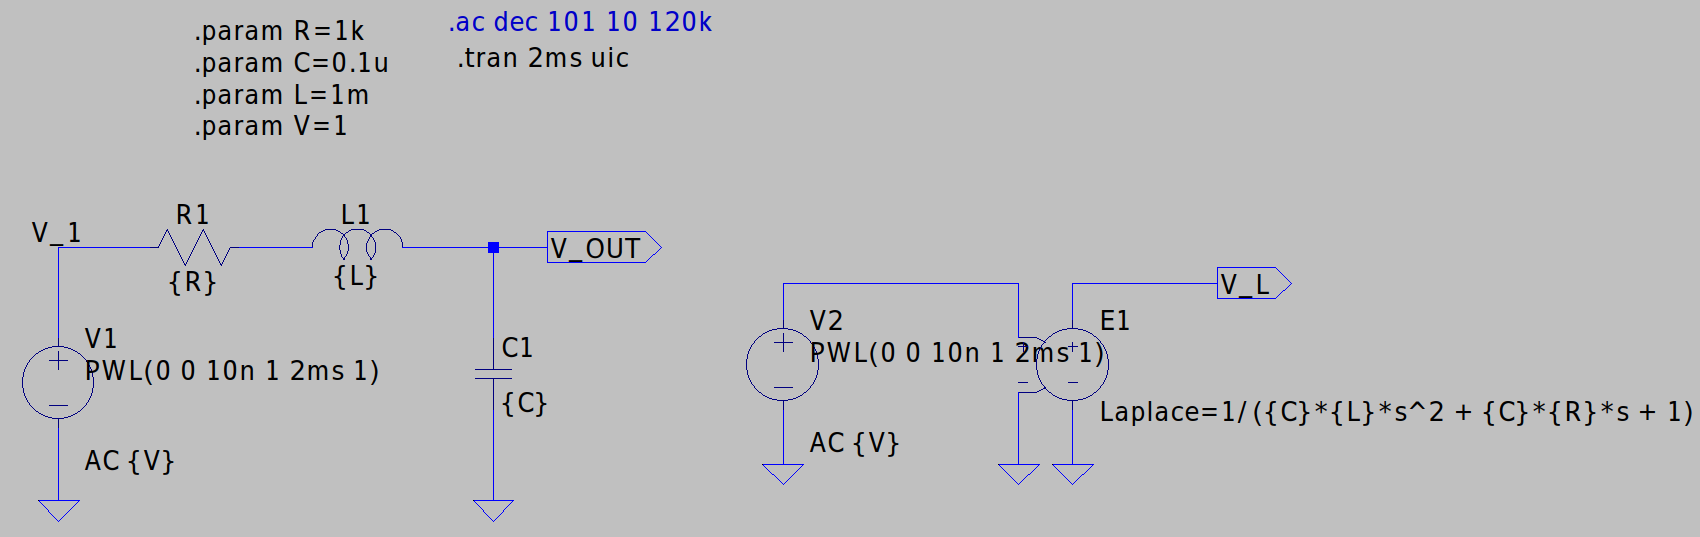
\includegraphics[width=1\textwidth, height=0.4\textheight]{assets/rlc-unit-step-sim.png}
    \caption{Unit Step Response Simulation Setup}
    \label{fig:unit_step_response}
\end{figure}

\newpage
\thispagestyle{plain}

\begin{figure}[h]
    \centering
    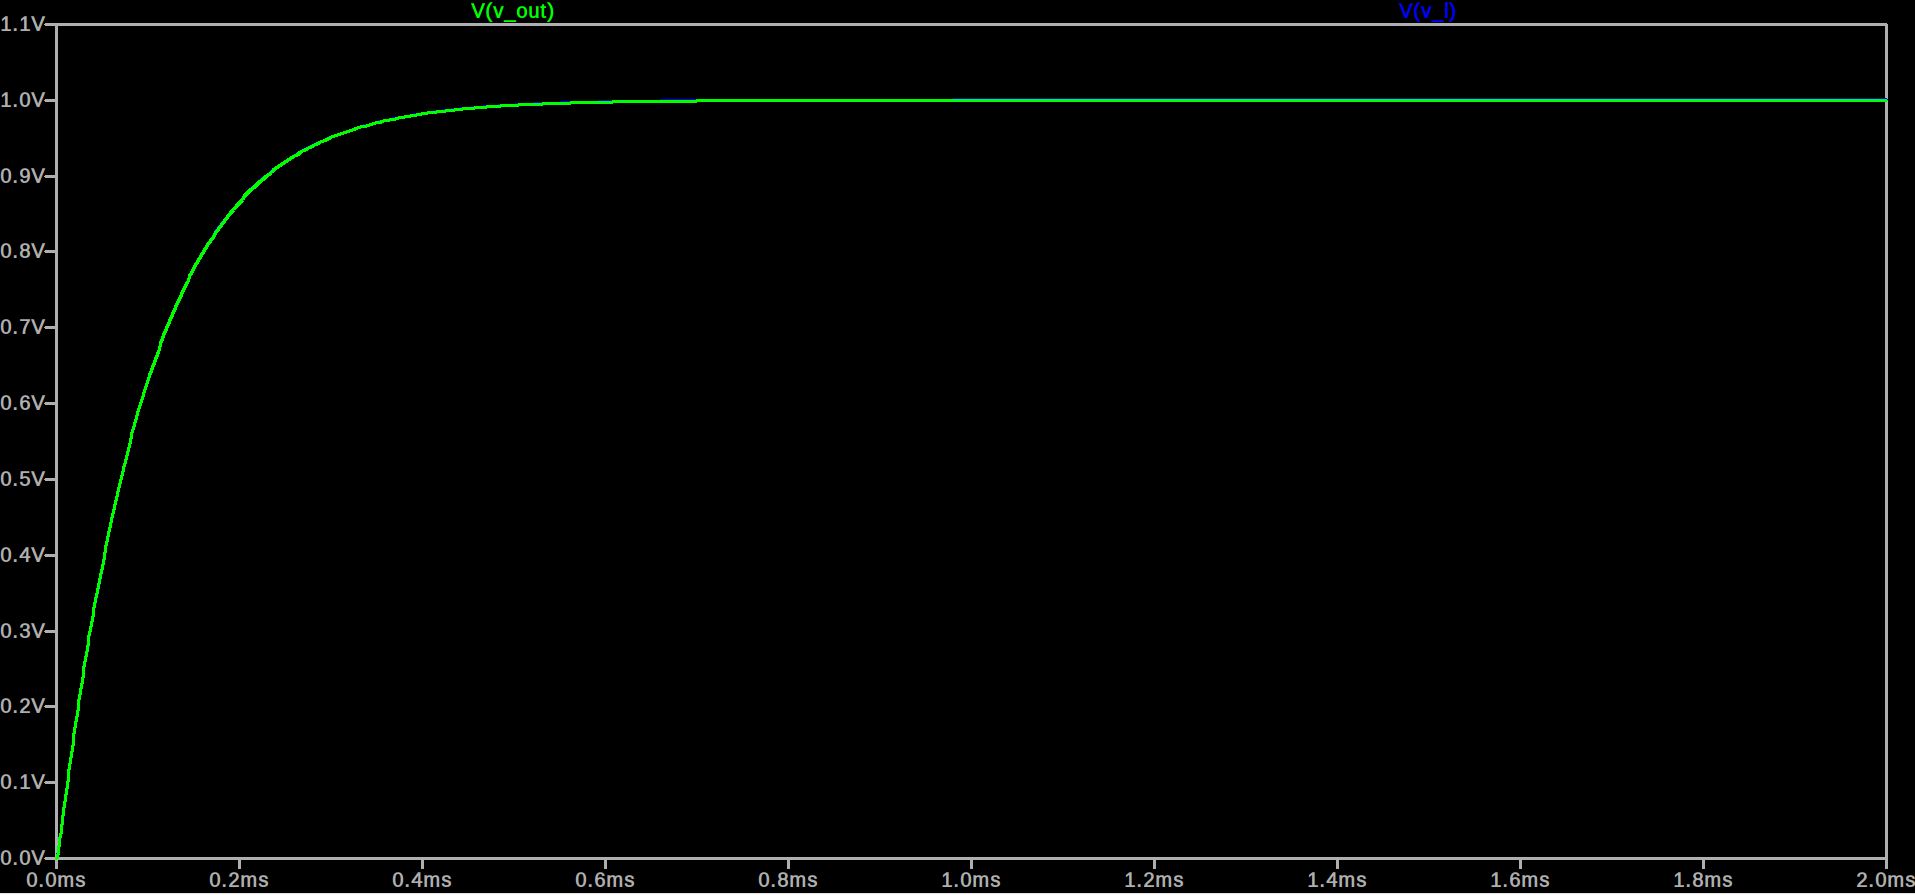
\includegraphics[width=1\textwidth]{assets/rlc-unit-step-sim-v-out.png}
    \caption{$V_{out}$ Unit Step Response}
    \label{fig:rlc_v_out_unit_step_response}
\end{figure}

\begin{figure}[h]
    \centering
    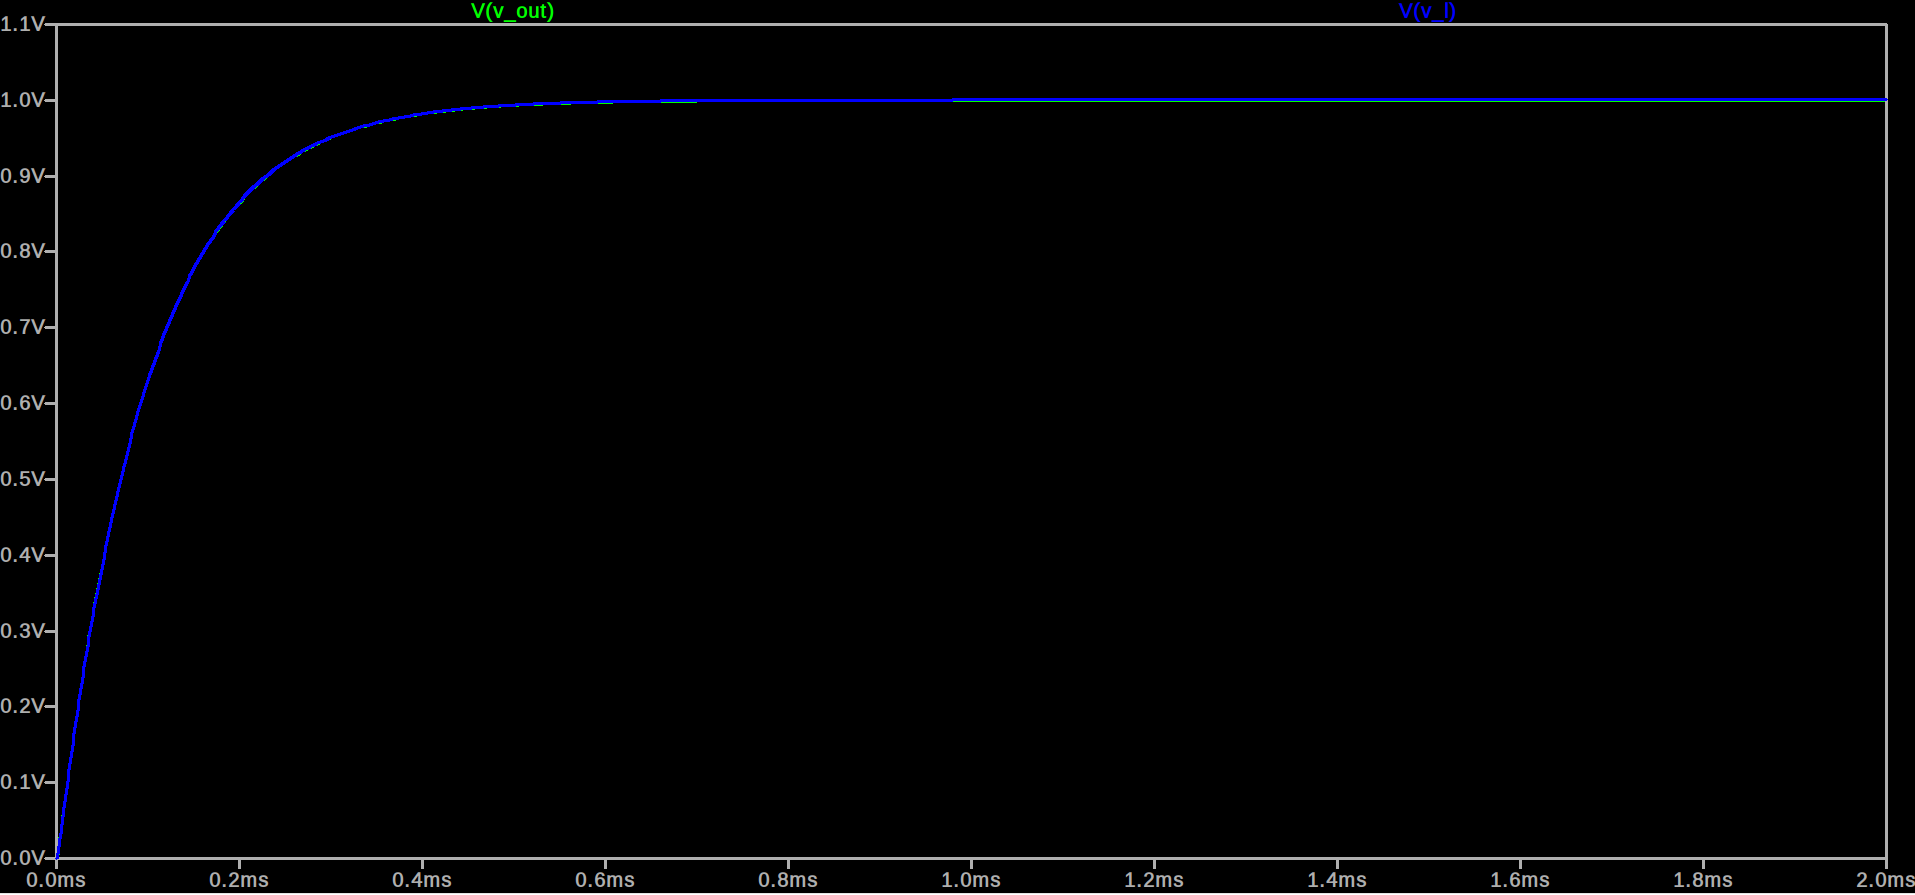
\includegraphics[width=1\textwidth]{assets/rlc-unit-step-sim-v-laplace.png}
    \caption{$H_{V}(s)$ Transient Response}
    \label{fig:rlc_v_laplace_unit_step_response}
\end{figure}

As shown in Figure \ref{fig:rlc_v_out_unit_step_response}, output voltage matches the transfer function $H_{V}(s)$ as shown in Figure \ref{fig:rlc_v_laplace_unit_step_response}.

\newpage
\thispagestyle{plain}

\subsection{Experimental Analysis}

In the first task, a circuit consisting of $1k\Omega$, $1mH$, and $1\mu F$ is constructed just as in Figure~\ref{fig:q1-circ}. Later a sine wave of $1V_{pp}$ is generated with different frequency values; $50Hz$, $500Hz$, $2kHz$, $5kHz$, $30kHz$, and $100kHz$. Output waves and the phase difference of the input and output of the circuit with corresponding frequency are observed and measured. 

\begin{figure}[h]
    \centering
    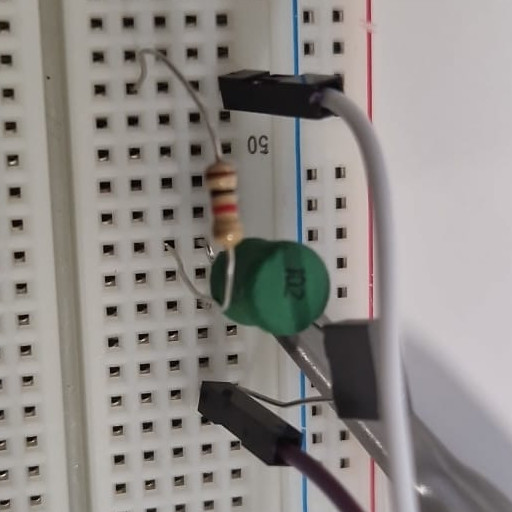
\includegraphics[width=0.5\textwidth]{assets/exp/q1-circ.jpeg}
    \caption{RLC Circuit}
    \label{fig:q1-circ}
\end{figure}

The output and input waveforms are visible in the figures below with frequencies $50Hz$, $500Hz$, $2kHz$, $5kHz$, $30kHz$, and $100kHz$ respectively. Channel 1 is output and channel 2 is input.

\begin{figure}[h]
    \centering
    \begin{minipage}{0.5\textwidth}
        \includegraphics[width=0.9\textwidth , height=0.2\textheight]{assets/exp/q1-50Hz-1vpp-comp.jpeg}
        \caption{Q1 50Hz Input-Output Comparasion}
        \label{fig:q1-50Hz-1vpp-comp}
    \end{minipage}%
    \begin{minipage}{0.5\textwidth}
        \includegraphics[width=0.9\textwidth , height=0.2\textheight]{assets/exp/q1-500Hz-1vpp-comp.jpeg}
        \caption{Q1 500Hz Input-Output Comparasion}
        \label{fig:q1-500Hz-1vpp-comp}
    \end{minipage}
\end{figure}

\newpage
\thispagestyle{plain}

\begin{figure}[h]
    \centering
    \begin{minipage}{0.5\textwidth}
        \includegraphics[width=0.9\textwidth , height=0.2\textheight]{assets/exp/q1-2kHz-1vpp-comp.jpeg}
        \caption{Q1 2kHz Input-Output Comparasion}
        \label{fig:q1-2kHz-1vpp-comp}
    \end{minipage}%
    \begin{minipage}{0.5\textwidth}
        \includegraphics[width=0.9\textwidth , height=0.2\textheight]{assets/exp/q1-5kHz-1vpp-comp.jpeg}
        \caption{Q1 5kHz Input-Output Comparasion}
        \label{fig:q1-5kHz-1vpp-comp}
    \end{minipage}
    \begin{minipage}{0.5\textwidth}
        \includegraphics[width=0.9\textwidth , height=0.2\textheight]{assets/exp/q1-30kHz-1vpp-comp.jpeg}
        \caption{Q1 30kHz Input-Output Comparasion}
        \label{fig:q1-30kHz-1vpp-comp}
    \end{minipage}%
    \begin{minipage}{0.5\textwidth}
        \includegraphics[width=0.9\textwidth , height=0.2\textheight]{assets/exp/q1-100kHz-1vpp-comp.jpeg}
        \caption{Q1 100kHz Input-Output Comparasion}
        \label{fig:q1-100kHz-1vpp-comp}
    \end{minipage}
\end{figure}

After that, to measure the phase difference, cursor function of the oscilloscope is opened and a cursor on each channels are placed. Time difference between the zero points of each channel is measured by the machine and it is put into the eq.~\ref{eq:phase_diff} to calculate the phase difference.The results are written down in the descriptions of each figure with the corresponding frequency.

\begin{equation} \label{eq:phase_diff}
    \phi = 360^{\circ} \times \Delta t \times f
\end{equation}

\begin{figure}[h]
    \centering
    \begin{minipage}{0.5\textwidth}
        \includegraphics[width=0.9\textwidth , height=0.15\textheight]{assets/exp/q1-50Hz-1vpp-phase.jpeg}
        \caption{Q1 50Hz, $9^{\circ}$ Phase Difference}
        \label{fig:q1-50Hz-1vpp-phase}
    \end{minipage}%
    \begin{minipage}{0.5\textwidth}
        \includegraphics[width=0.9\textwidth , height=0.15\textheight]{assets/exp/q1-500Hz-1vpp-phase.jpeg}
        \caption{Q1 500Hz, $27^{\circ}$ Phase Difference}
        \label{fig:q1-500Hz-1vpp-phase}
    \end{minipage}
\end{figure}

\newpage
\thispagestyle{plain}

\begin{figure}[h]
    \centering
    \begin{minipage}{0.5\textwidth}
        \includegraphics[width=0.9\textwidth , height=0.2\textheight]{assets/exp/q1-2kHz-1vpp-phase.jpeg}
        \caption{Q1 2kHz, $70.56^{\circ}$ Phase Difference}
        \label{fig:q1-2kHz-1vpp-phase}
    \end{minipage}%
    \begin{minipage}{0.5\textwidth}
        \includegraphics[width=0.9\textwidth , height=0.2\textheight]{assets/exp/q1-5kHz-1vpp-phase.jpeg}
        \caption{Q1 5kHz, $75.6^{\circ}$ Phase Difference}
        \label{fig:q1-5kHz-1vpp-phase}
    \end{minipage}
    \begin{minipage}{0.5\textwidth}
        \includegraphics[width=0.9\textwidth , height=0.2\textheight]{assets/exp/q1-30kHz-1vpp-phase.jpeg}
        \caption{Q1 30kHz, $86.4^{\circ}$ Phase Difference}
        \label{fig:q1-30kHz-1vpp-phase}
    \end{minipage}
\end{figure}

Again, when it came to $100kHz$, the oscilloscope screen showed $126kHz$ instead. The calculations are done with each of these frequencies to make a comparison.

\begin{figure}[h]
    \centering
    \includegraphics[width=0.5\textwidth]{assets/exp/q1-100kHz-1vpp-signal.jpeg}
    \caption{Q1 100kHz Function Generator Signal}
    \label{fig:q1-100kHz-1vpp-signal}
\end{figure}

\newpage
\thispagestyle{plain}

By calculating, it is discovered that the frequency in the oscilloscope is incorrect because if there was a delay of $181.44^{\circ}$, the zero points of the input and output would almost be matching.
\begin{figure}[h]
    \centering
    \includegraphics[width=0.9\textwidth]{assets/exp/q1-100kHz-1vpp-phase.jpeg}
    \caption{Q1 100kHz, $144^{\circ}$ Phase Difference, 126kHz, $181.44^{\circ}$ Phase Difference}
    \label{fig:q1-100kHz-1vpp-phase}
\end{figure}


\newpage
\thispagestyle{plain}

\section{Op-Amp Circuit Analysis}

\subsection{Theoretical Analysis}

\subsubsection{Transfer Function Derivation}
In order to derive the voltage gain transfer function ($H_{V}(s)$), we must first convert the circuit from time domain to the s-domain. The circuit is shown in Figure \ref{fig:op_amp_circuit}.

\begin{figure}[h]
    \centering
    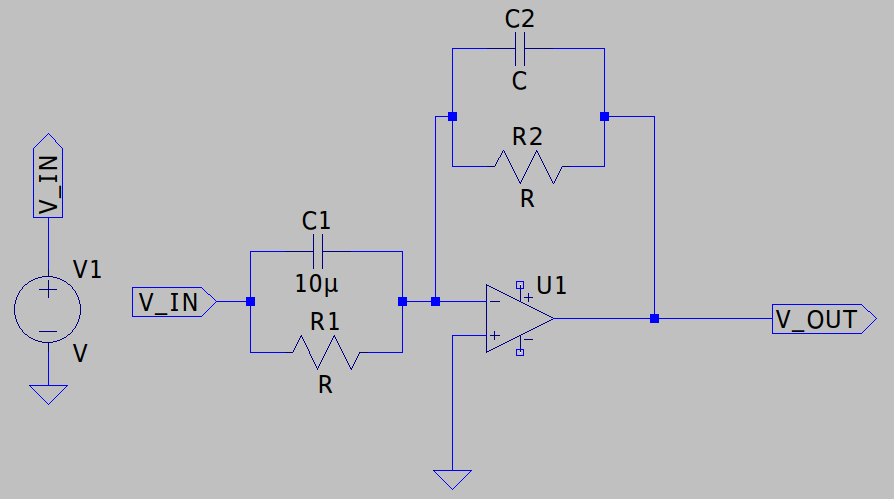
\includegraphics[width=1\textwidth]{assets/opamp-circ.png}
    \caption{Op-Amp Circuit}
    \label{fig:op_amp_circuit}
\end{figure}

\noindent Expected transfer function is $H_{V}(s) = \frac{V_{o}}{V_{i}} = -\frac{s+1000}{2(s+4000)}$:


\begin{align*}
    \text{let } Z_1 &= \frac{R_1}{1 + C_1 R_1 s} \\
    \text{let } Z_2 &= \frac{R_2}{1 + C_2 R_2 s} \\
    \frac{V_{in}}{Z_1} &= -\frac{V_{out}}{Z_2}\\
    V_{out} &= -\frac{Z_2}{Z_1} V_{in} \\
    \implies H_{V}(s) &= -\frac{Z_2}{Z_1} = -\frac{s+1000}{2(s+4000)} \\
    \frac{s+1000}{2(s+4000)} &= \frac{C_1}{C_2}\cdot \left[ \frac{s + \frac{1}{R_1 C_1}}{s + \frac{1}{R_2 C_2}} \right] \\
    \implies C_1 &= 10\mu F, C_2 = 20\mu F, R_1 = 100\Omega, R_2 = 12.5\Omega
\end{align*}

\newpage
\thispagestyle{plain}

Using these values, bode plot of the circuit and transfer function is shown below:

\begin{figure}[h]
    \centering
    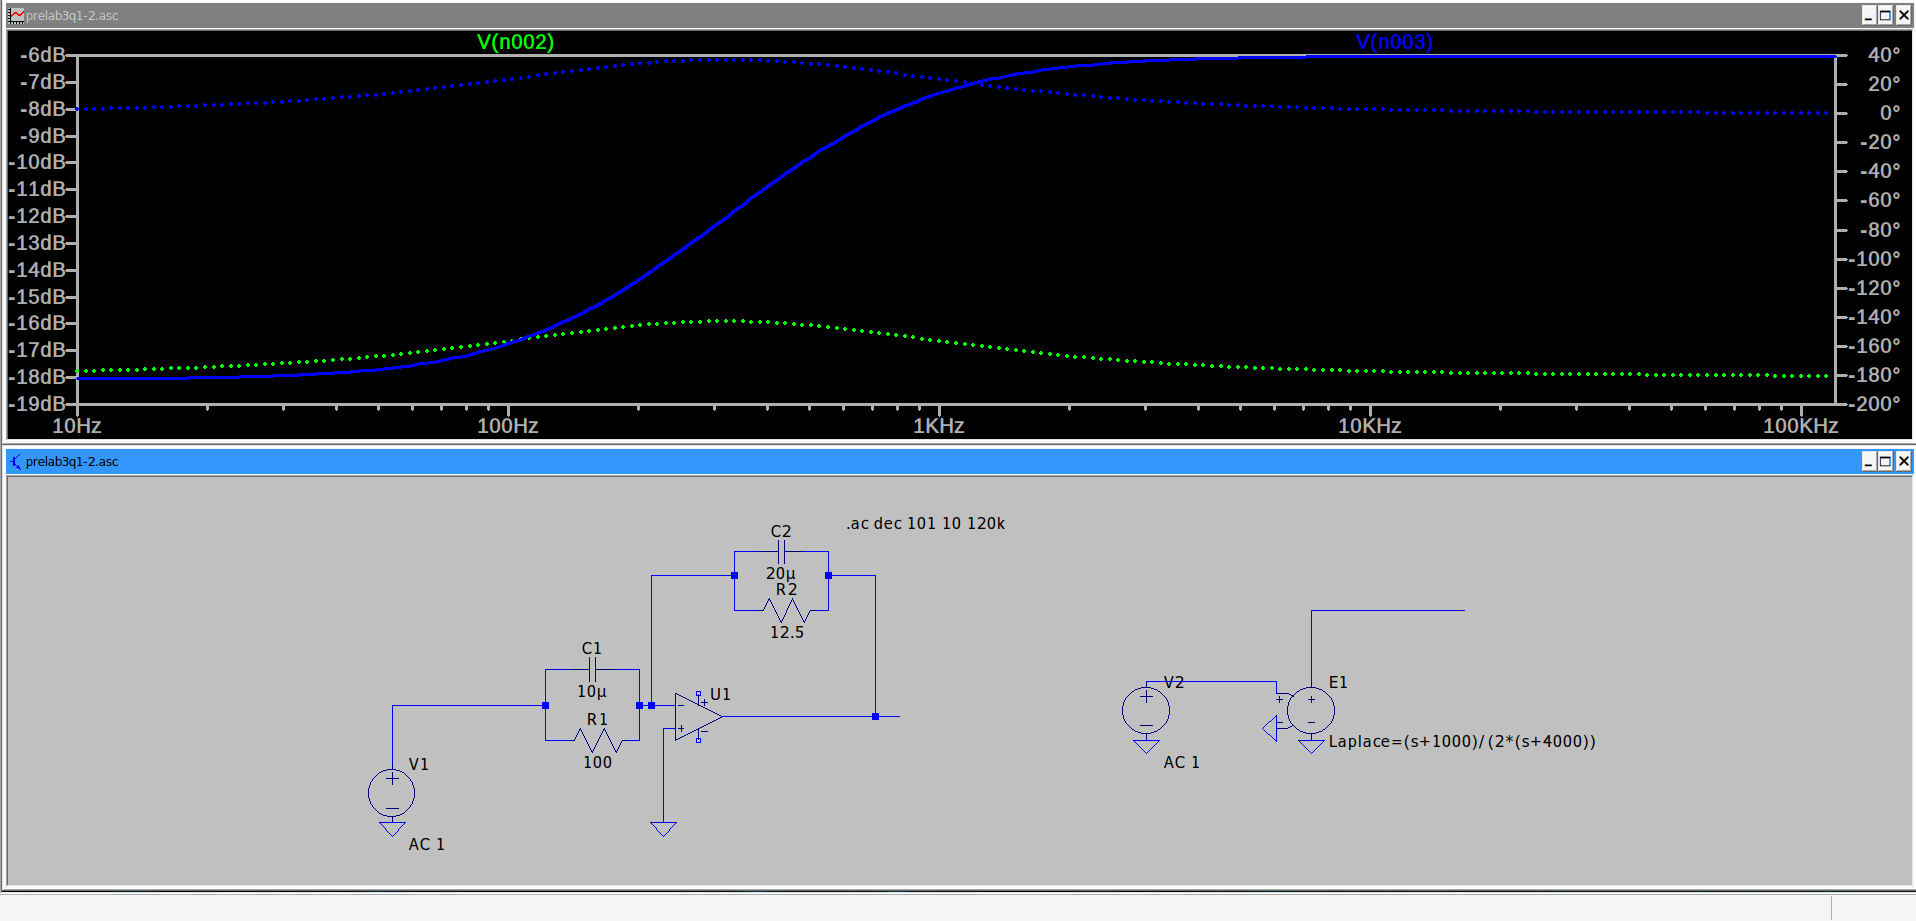
\includegraphics[width=1\textwidth]{assets/q2-fixed.png}
    \caption{$V_{out}$ \& $H(s)$ Bode Plot}
    \label{fig:op_amp_v_out_bode_plot}
\end{figure}

As can be seen in Figure \ref{fig:op_amp_v_out_bode_plot}, output and transfer function bode plots are matching.

\begin{figure}[h]
    \centering
    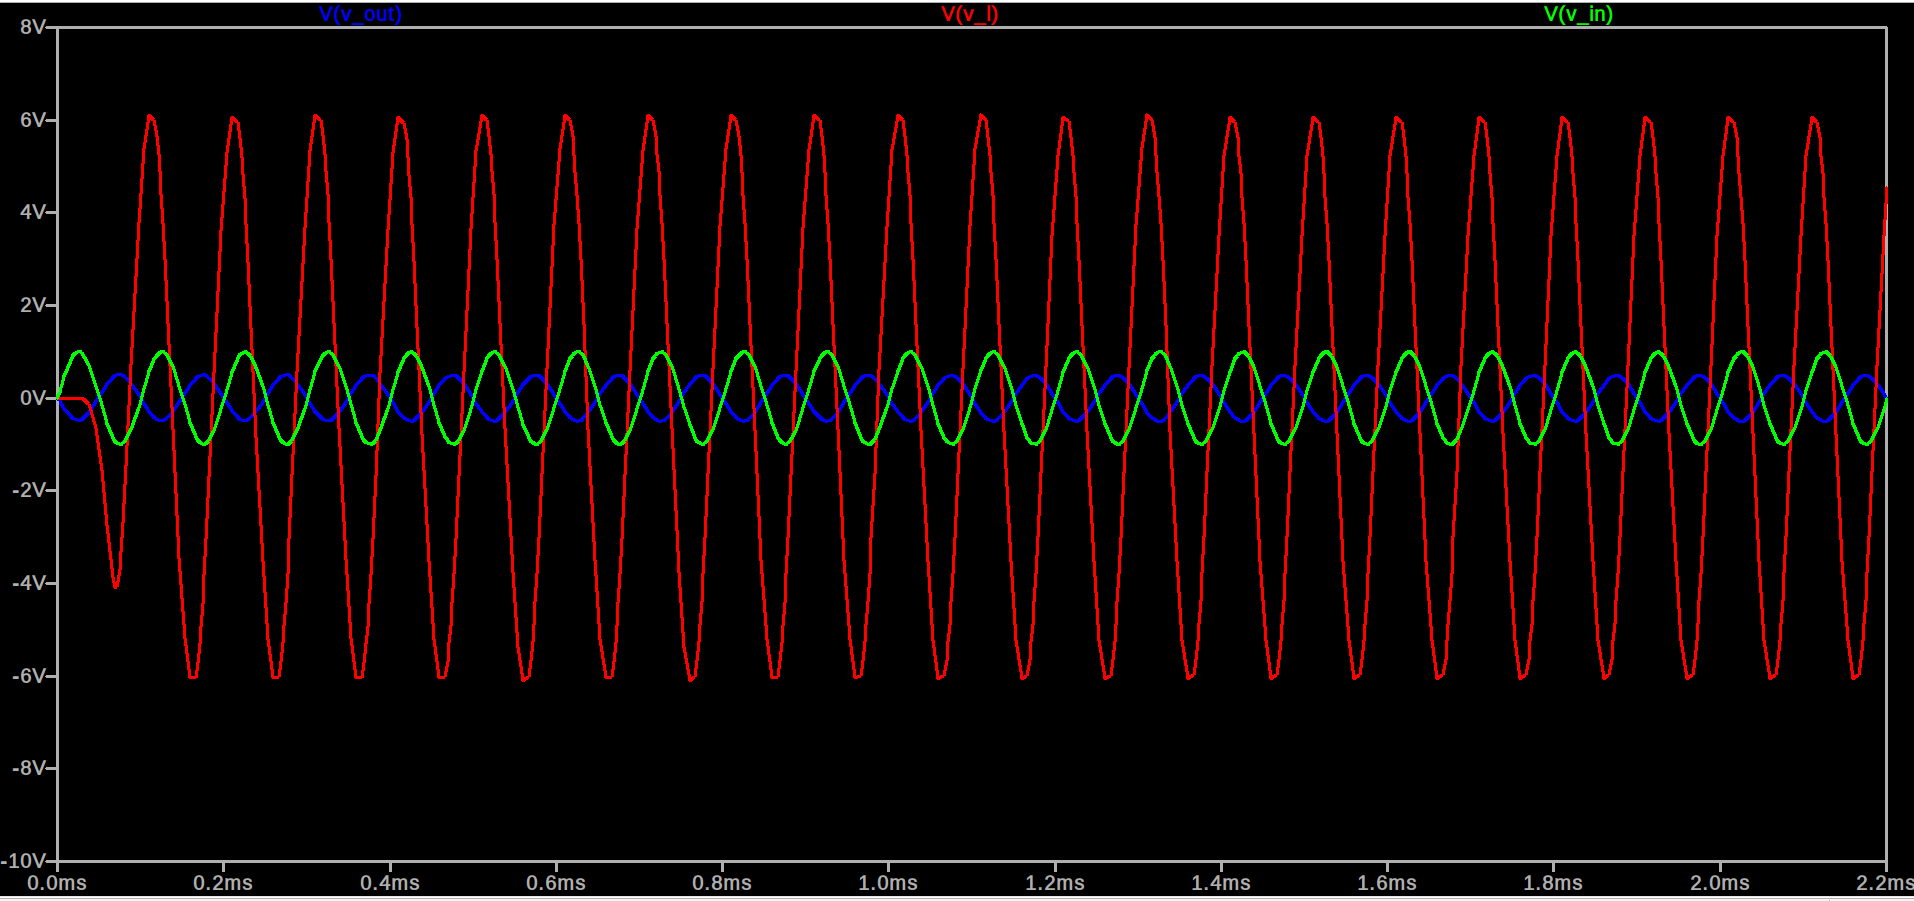
\includegraphics[width=1\textwidth]{assets/opamp-10k.png}
    \caption{$V_{in}$, $V_{out}$ \& $H(s)$ Plot @ $10kHz$}
    \label{fig:op_amp_out_10k}
\end{figure}

\begin{figure}[h]
    \centering
    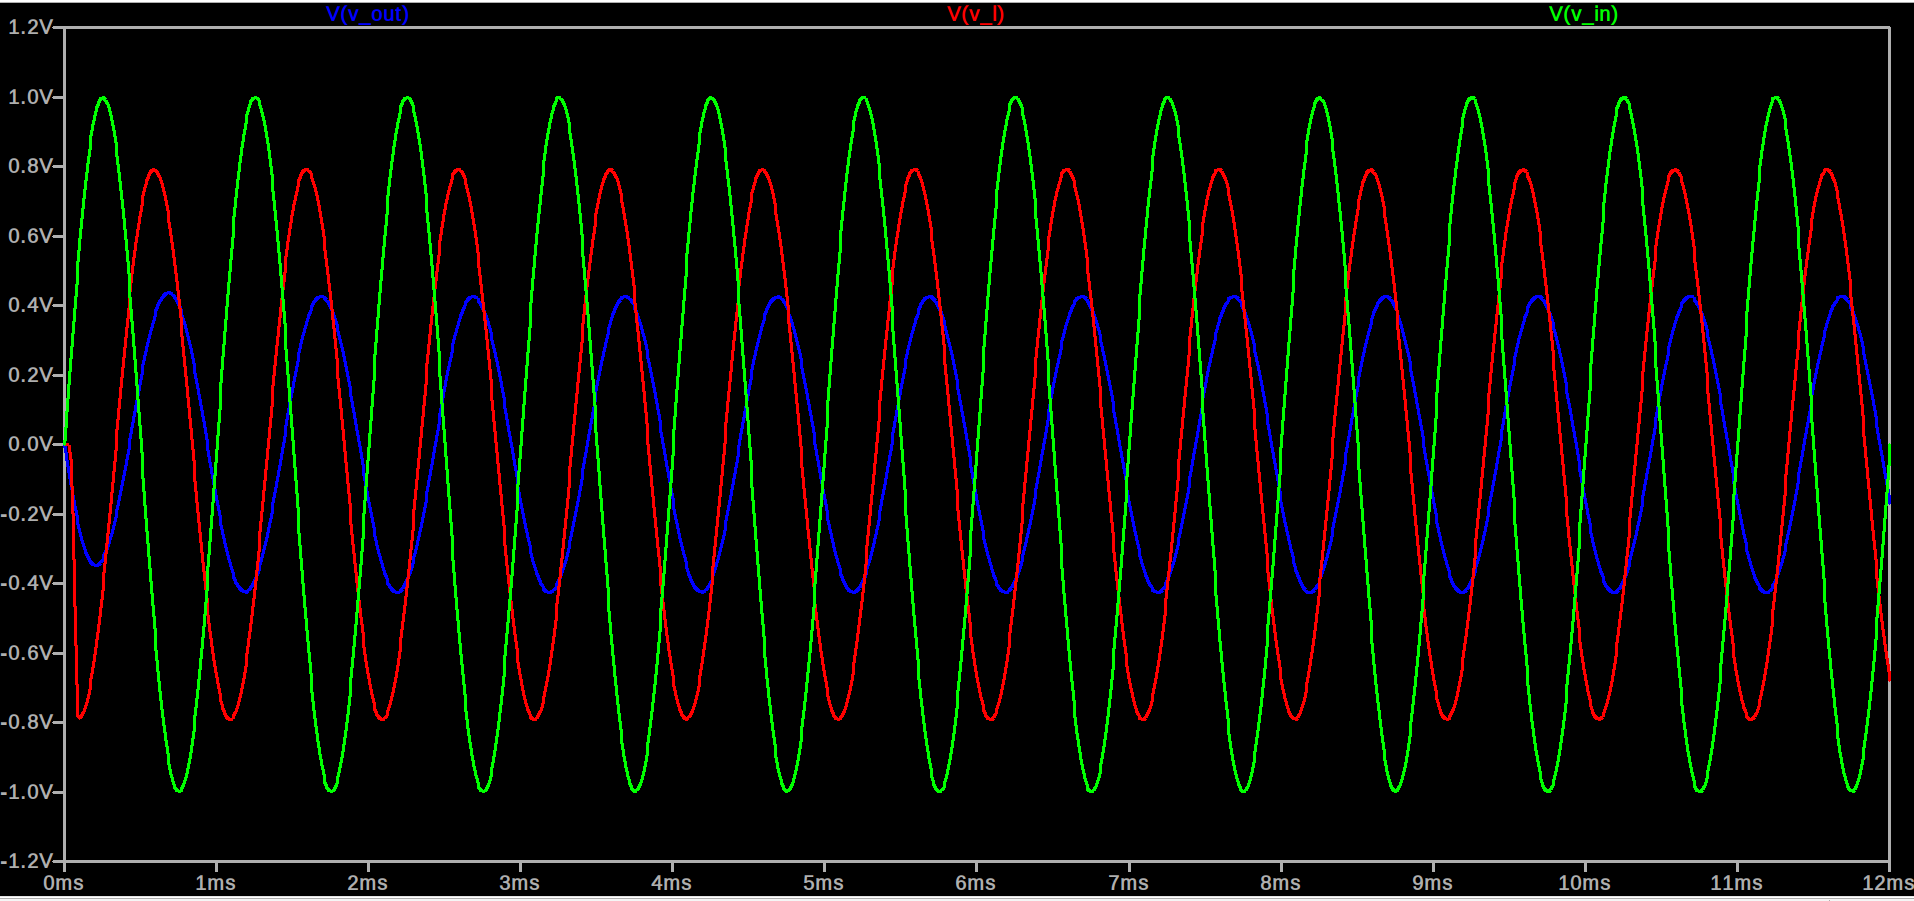
\includegraphics[width=1\textwidth]{assets/opamp-1k.png}
    \caption{$V_{in}$, $V_{out}$ \& $H(s)$ Plot @ $1kHz$}
    \label{fig:op_amp_out_1k}
\end{figure}

\newpage
\thispagestyle{plain}

\begin{figure}[h]
    \centering
    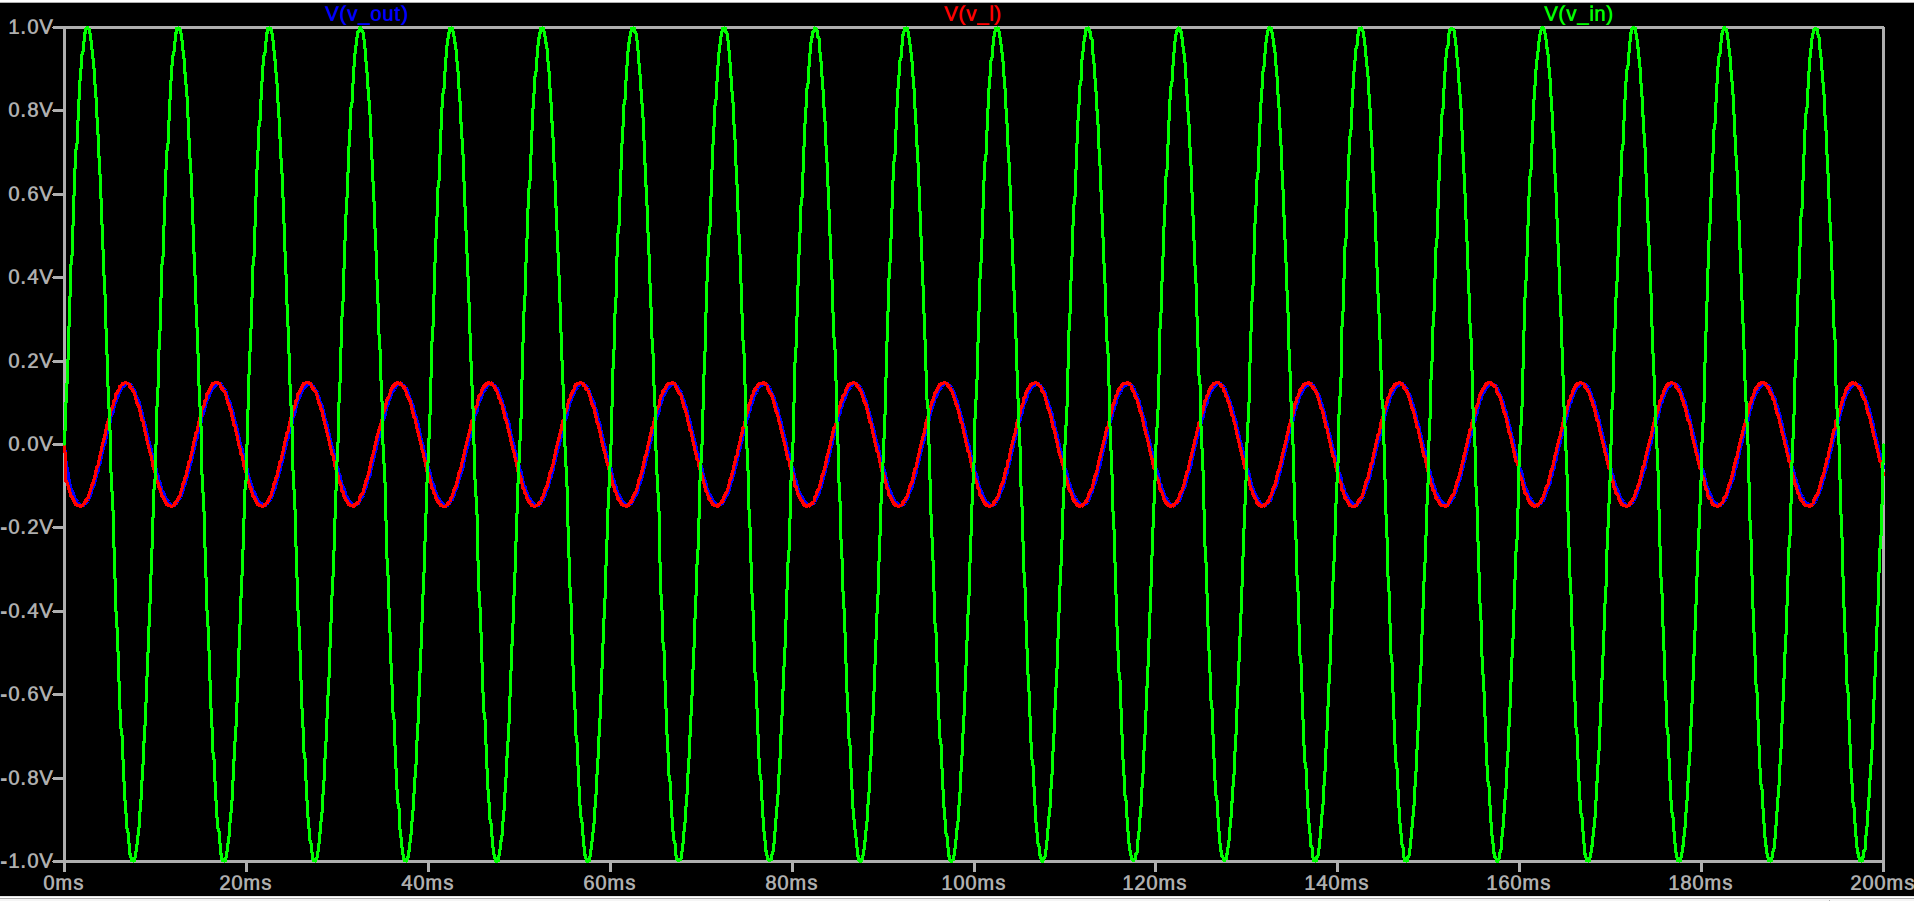
\includegraphics[width=1\textwidth]{assets/opamp-100.png}
    \caption{$V_{in}$, $V_{out}$ \& $H(s)$ Plot @ $100Hz$}
    \label{fig:op_amp_out_100}
\end{figure}

Plots seen in Figures \ref{fig:op_amp_out_10k}, \ref{fig:op_amp_out_1k}, and \ref{fig:op_amp_out_100} show the input and output voltages at $10kHz$, $1kHz$, and $100Hz$ respectively. These graphs confirms the bode plot in Figure \ref{fig:op_amp_v_out_bode_plot}.

\newpage
\thispagestyle{plain}

\subsection{Experimental Analysis}

In order to confirm the theoretical analysis, the circuit shown in Figure \ref{fig:q2-circ} is constructed. A sine wave of $1V_{pp}$ is generated with different frequency values; $1kHz$ and $2kHz$. Output waves and the phase difference of the input and output of the circuit with corresponding frequency are observed and measured.

\begin{figure}[h]
    \centering
    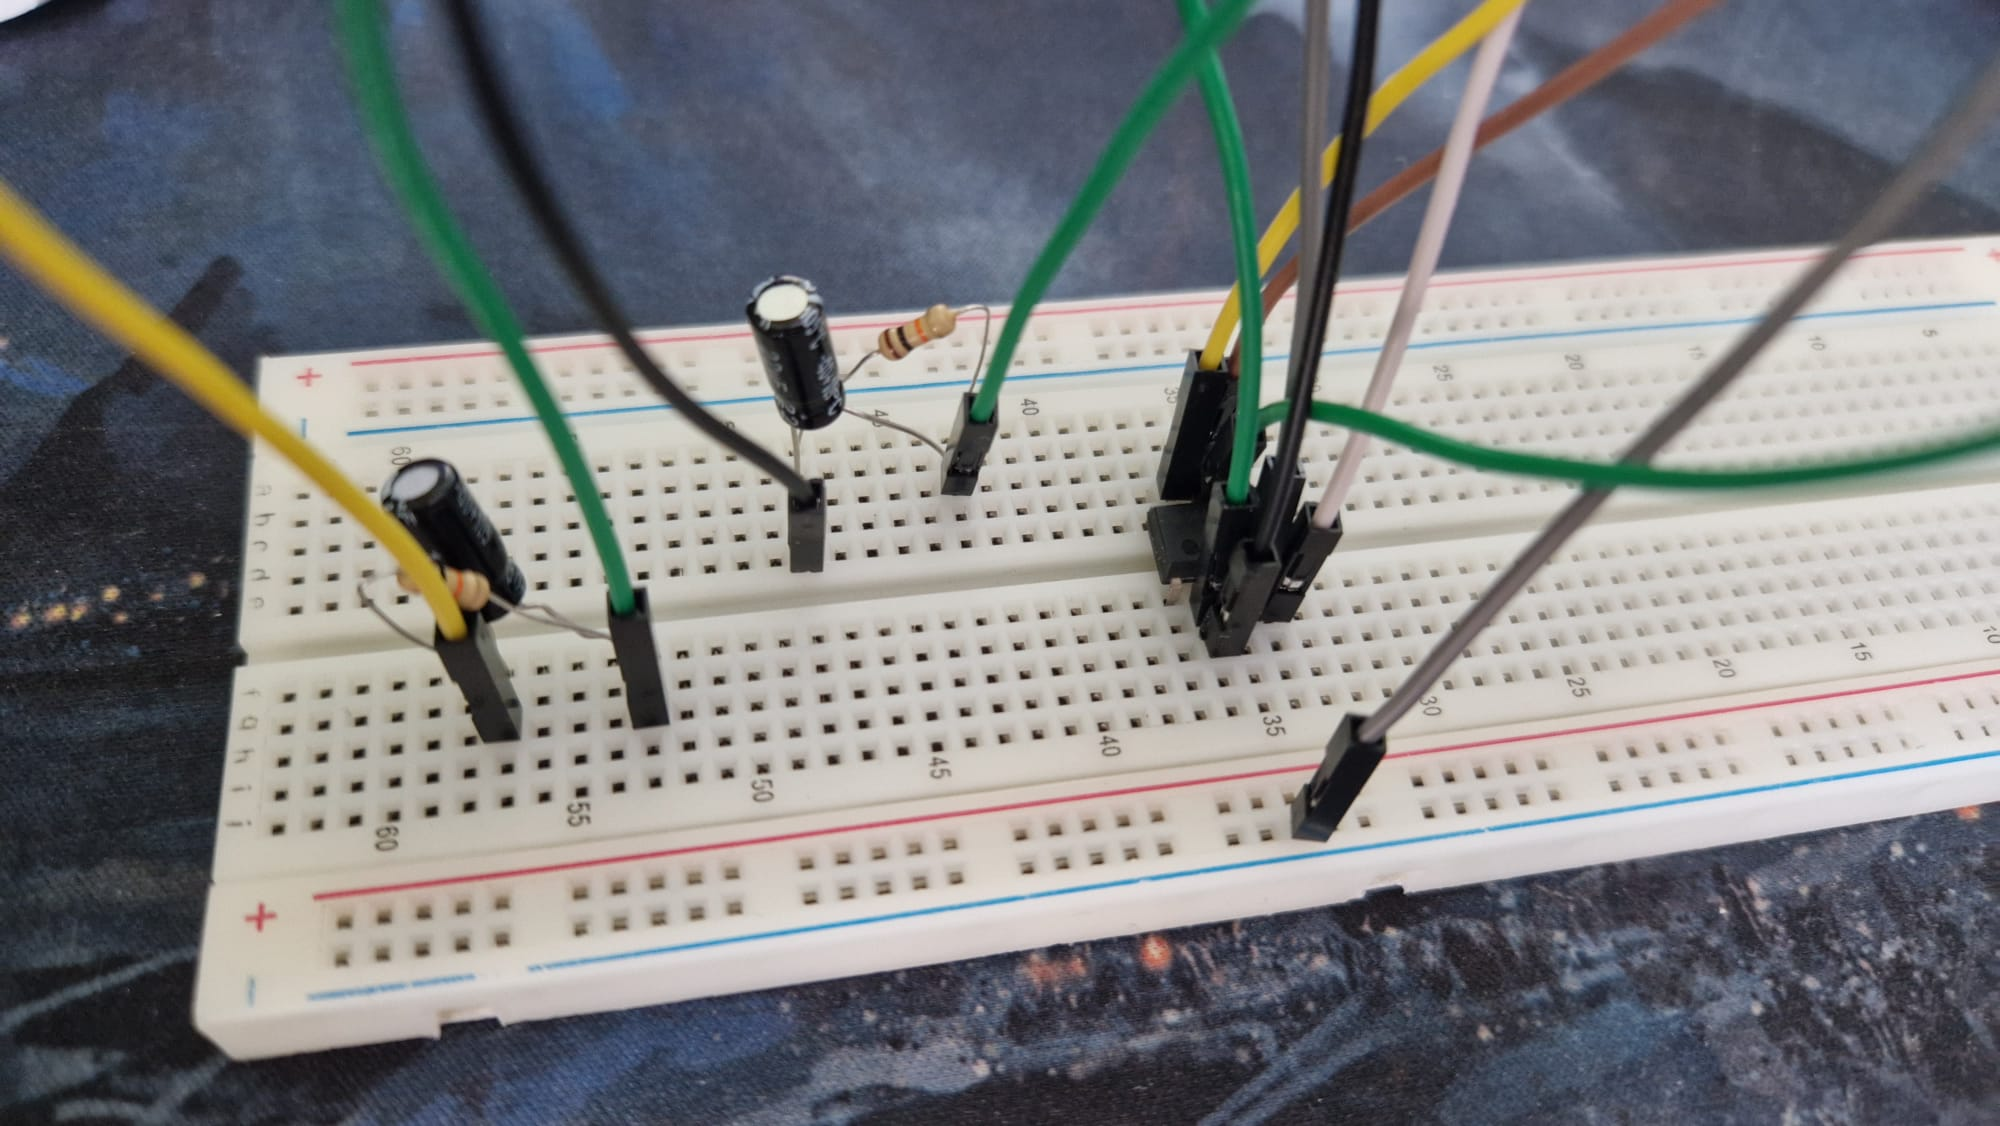
\includegraphics[width=0.5\textwidth]{assets/exp/q2-circ.jpeg}
    \caption{Op-Amp Circuit}
    \label{fig:q2-circ}
\end{figure}

\begin{figure}[h]
    \centering
    \begin{minipage}{0.5\textwidth}
        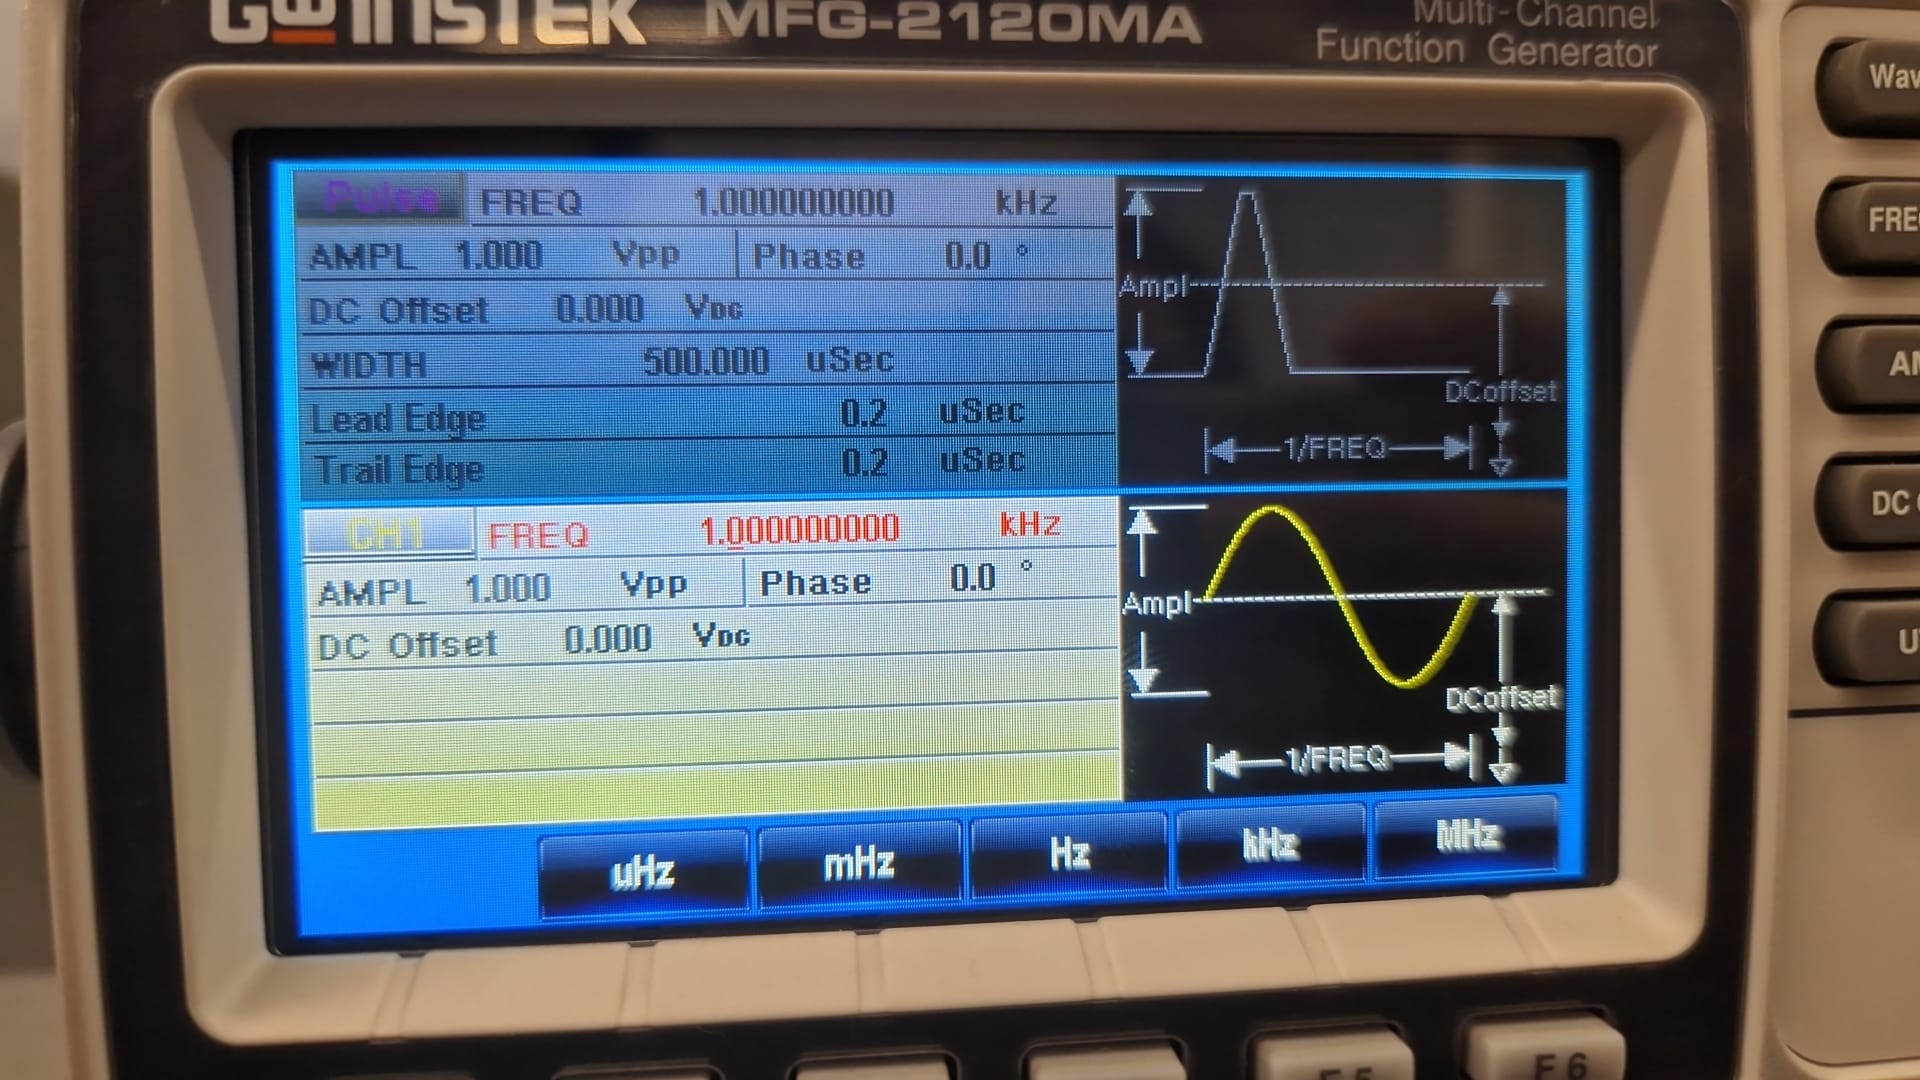
\includegraphics[width=0.9\textwidth , height=0.2\textheight]{assets/exp/q2-1khz-1vpp-signal.jpeg}
        \caption{Q2 1kHz Function Generator Signal}
        \label{fig:q2-1khz-1vpp-signal}
    \end{minipage}%
    \begin{minipage}{0.5\textwidth}
        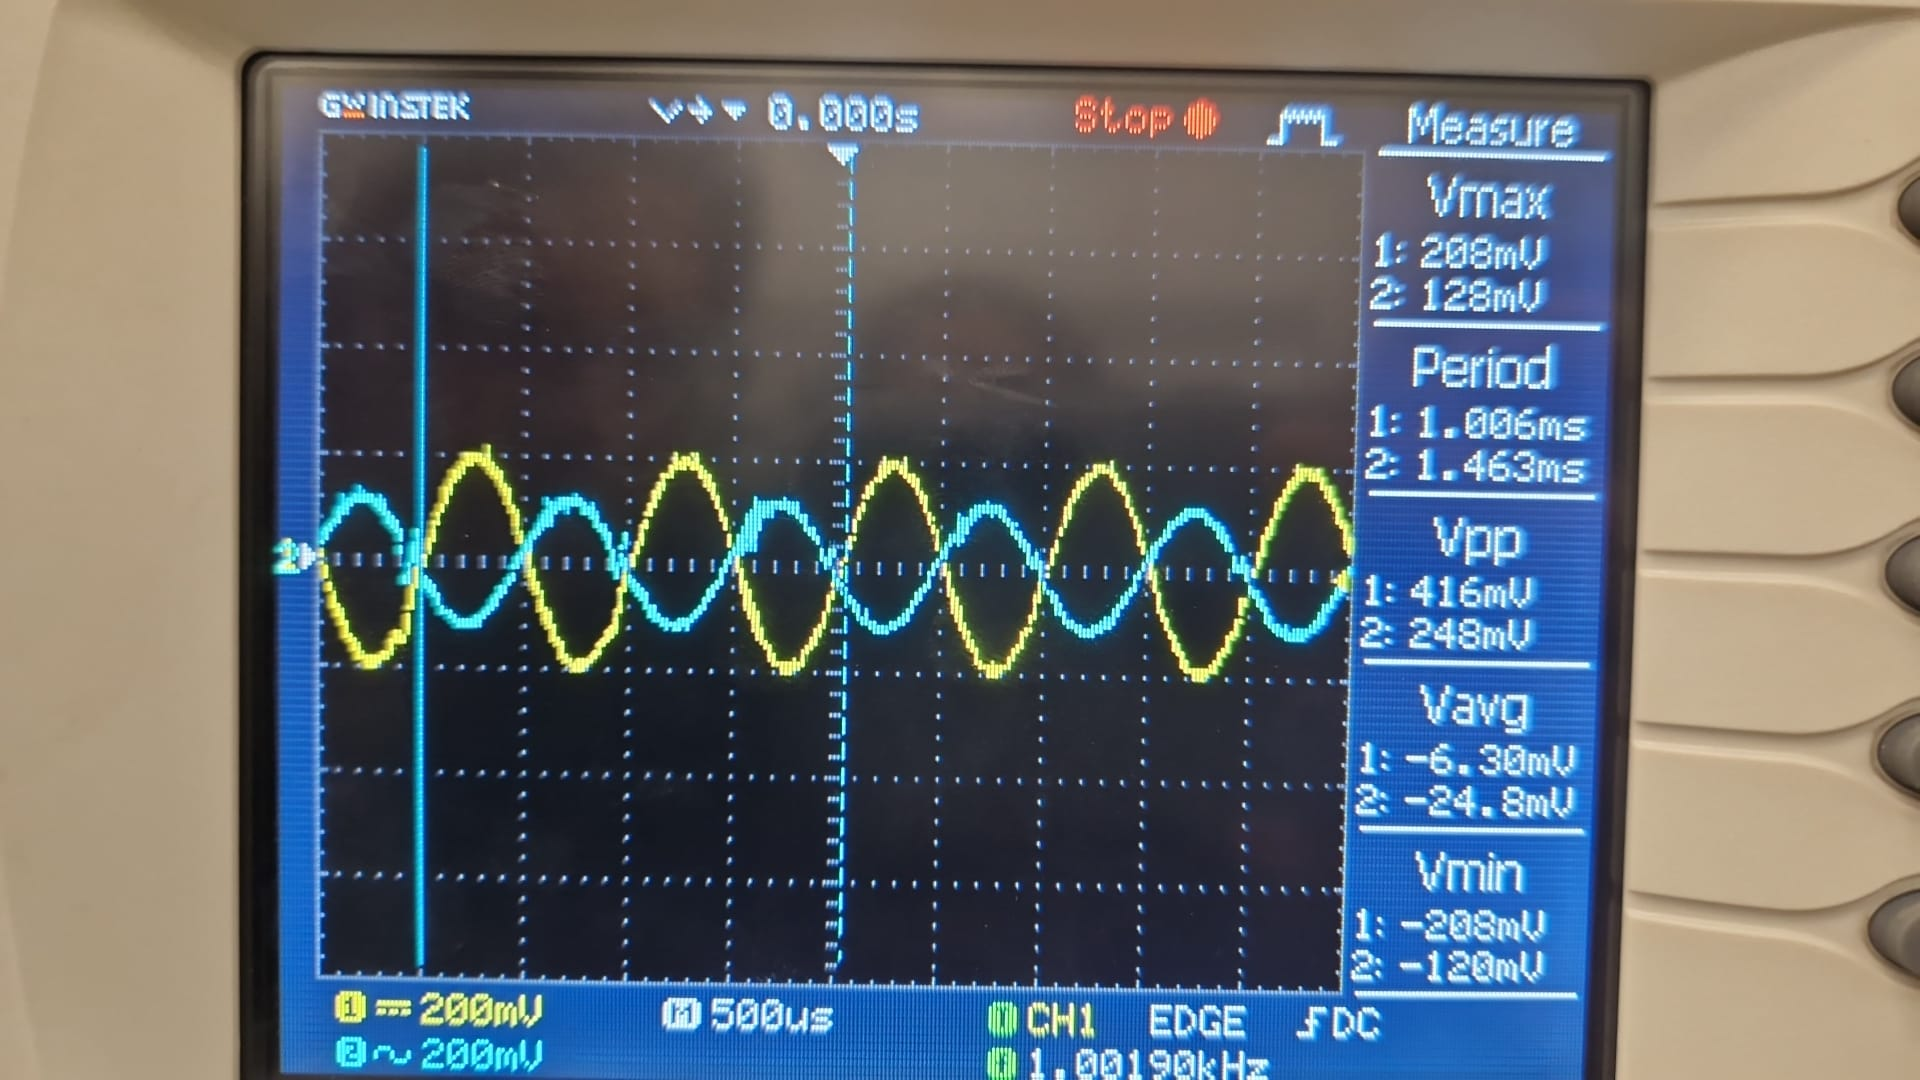
\includegraphics[width=0.9\textwidth , height=0.2\textheight]{assets/exp/q2-1khz-1vpp-comp.jpeg}
        \caption{Q2 1kHz Input-Output Comparasion}
        \label{fig:q2-1khz-1vpp-comp}
    \end{minipage}
    \begin{minipage}{0.5\textwidth}
        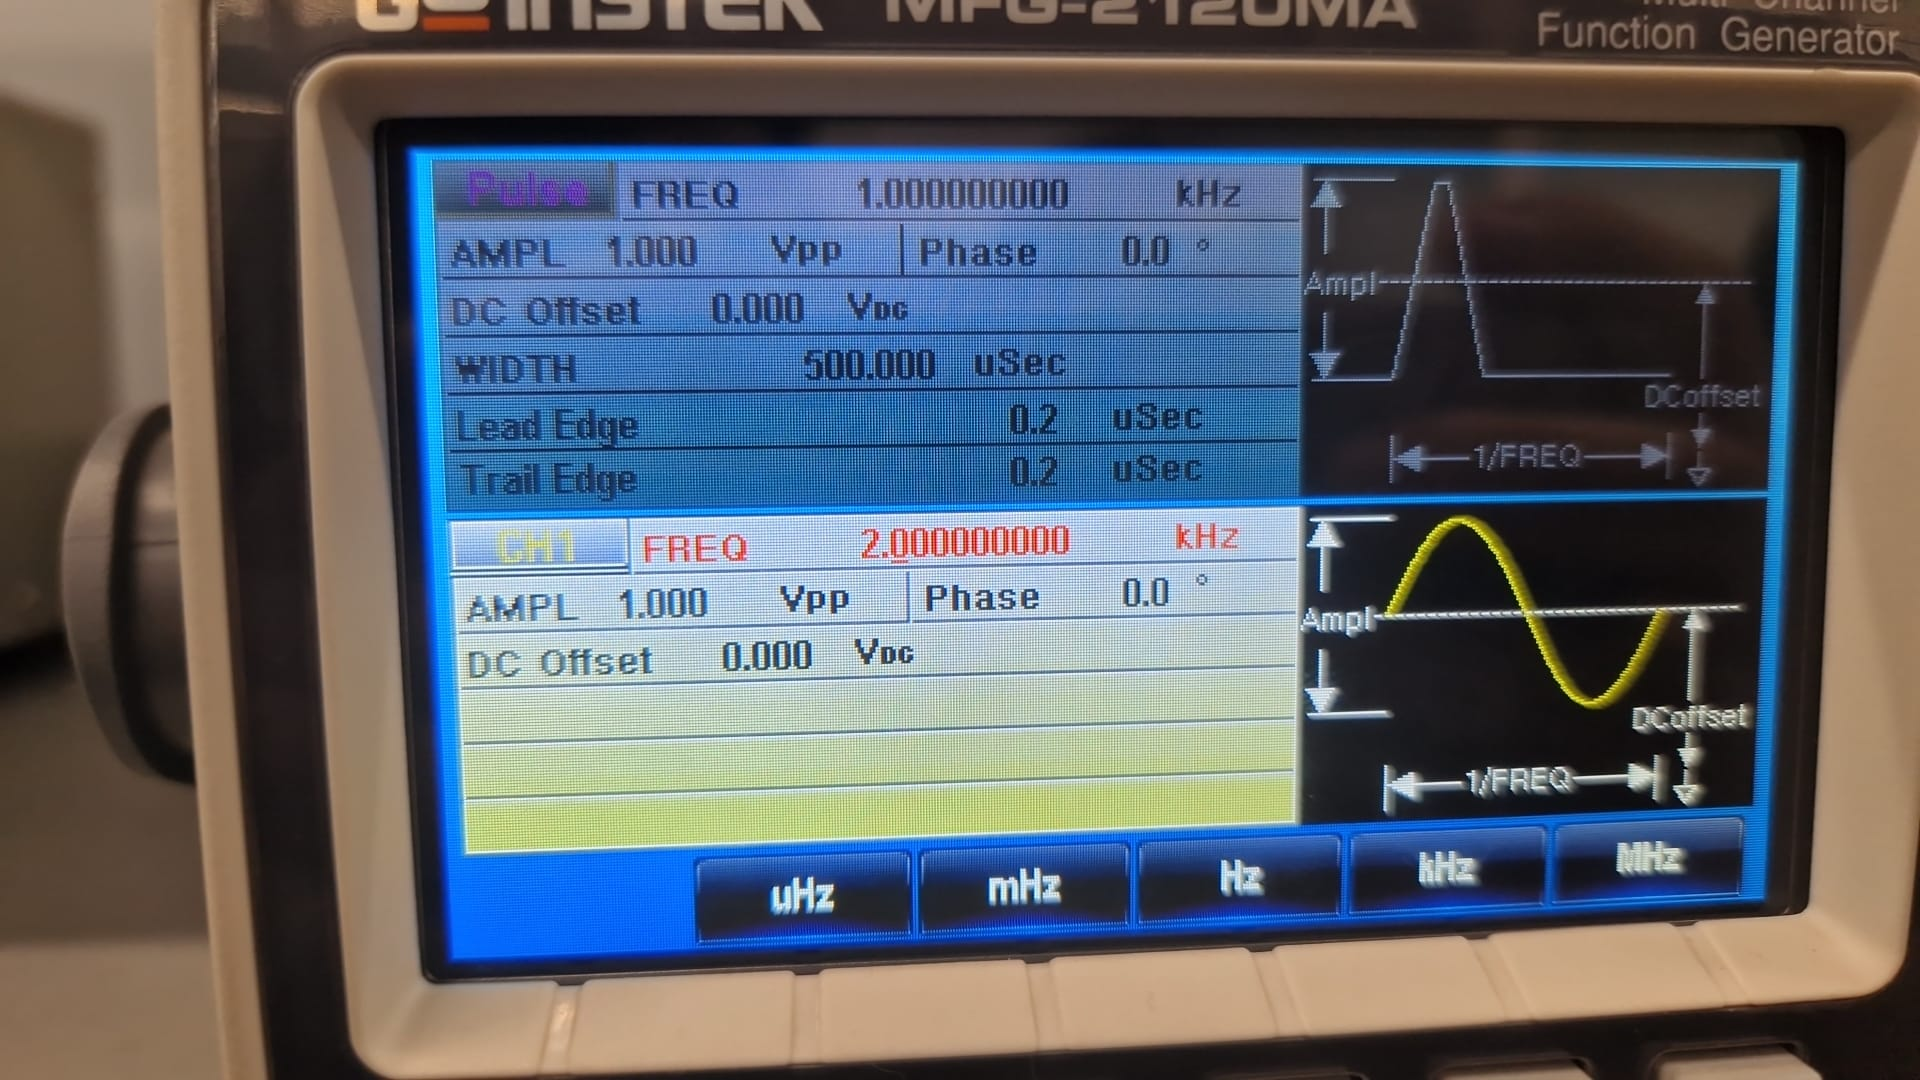
\includegraphics[width=0.9\textwidth , height=0.2\textheight]{assets/exp/q2-2khz-1vpp-signal.jpeg}
        \caption{Q2 2kHz Function Generator Signal}
        \label{fig:q2-2khz-1vpp-signal}
    \end{minipage}%
    \begin{minipage}{0.5\textwidth}
        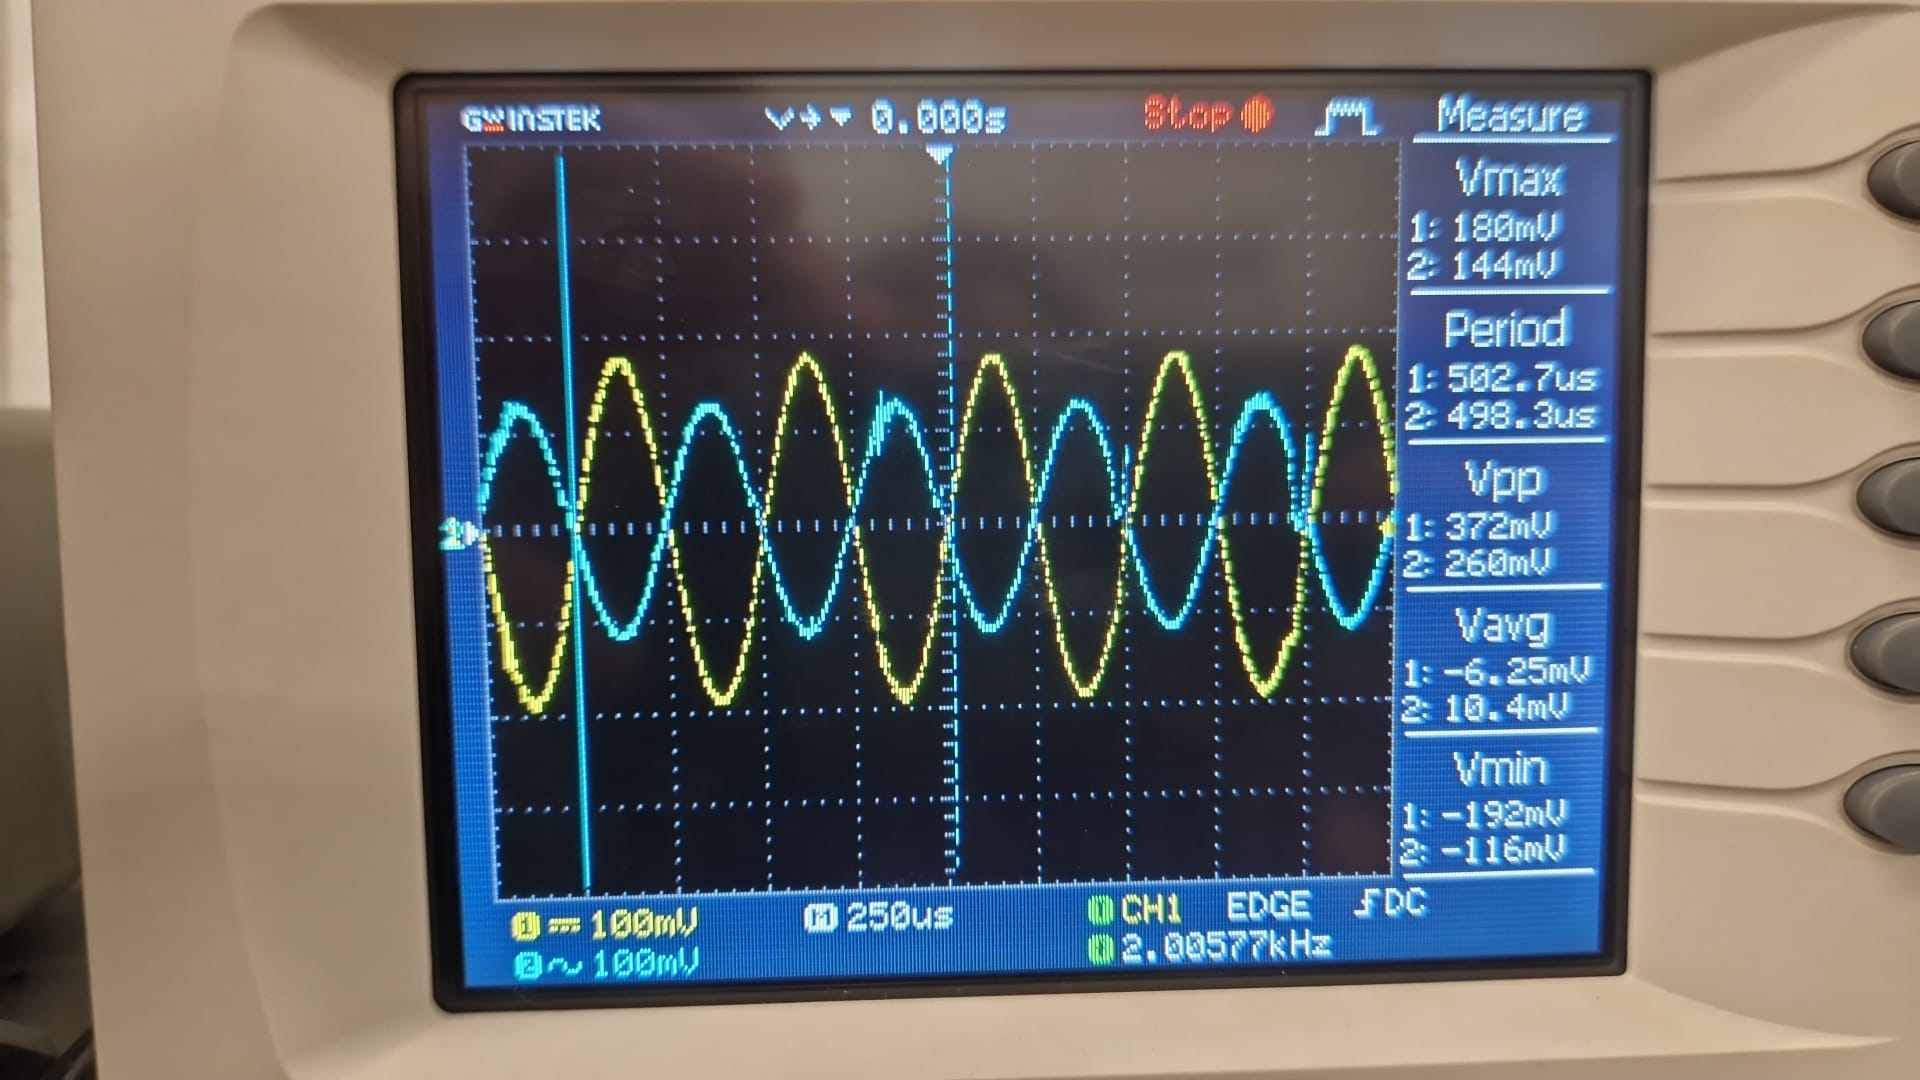
\includegraphics[width=0.9\textwidth , height=0.2\textheight]{assets/exp/q2-2khz-1vpp-comp.jpeg}
        \caption{Q2 2kHz Input-Output Comparasion}
        \label{fig:q2-2khz-1vpp-comp}
    \end{minipage}
\end{figure}

The transfer function and frequency response of the circuit coincide with the analyses predicted in the preliminary laboratory phase. It is also observed that the designed op-amp based active filter circuit exhibits the expected amplitude attenuation and phase shift in response to the applied 1kHz input signal.

	\chapter{Discussion}

\begin{itemize}
    \item \textbf{Comparison of Analytical and Simulated Results:} The derived transfer function $H(s)$ accurately predicted the frequency and transient responses observed in LTSpice simulations.
    \item \textbf{Frequency Response:} The AC Sweep analysis showed that Laplace transform and transfer functions are effective tools for analyzing frequency response that simplifies the process of determining the circuit's behavior at different frequencies.
    \item \textbf{Step Response:} The transient response of the circuit was analyzed using the step response of the circuit. The step response showed that the circuit is stable and has a fast response time.
    \item \textbf{Op-Amp Circuit Behavior:} The op-amp circuit was analyzed using the transfer function $H(s)$ and the transient response of the circuit. The circuit was found to be stable and had a fast response time. Poles and zeros of the transfer function were used to analyze the stability and characteristics of the circuit and it matched with the results.
\end{itemize}


	\chapter{Conclusion}

This lab demonstrated the effectiveness of the Laplace Transform and LTSpice simulations in analyzing and designing circuits. The step-by-step procedure validated theoretical predictions through simulation and experiment. The approach provided valuable insights into frequency and time-domain responses for RLC and op-amp circuits, highlighting the practical application of Laplace Transform in circuit analysis.

\end{document}
